\documentclass{beamer}

%% \documentclass[handout]{beamer}
%% % use this with the [handout] option to create handouts for the audience
%% \usepackage{pgfpages}
%% \pgfpagesuselayout{2 on 1}[a4paper,border shrink=5mm]

\mode<presentation>
{
  \usetheme{Diku}
% set this to your preferences:
  \setbeamercovered{invisible}
%  \setbeamercovered{transparent}
}

\usepackage{graphicx}
\usepackage{epic}

\usepackage{amsmath}
\usepackage{amssymb}
\usepackage{amsthm}

\newcommand{\basetop}[1]{\vtop{\vskip-1ex\hbox{#1}}}
\newcommand{\source}[1]{\let\thefootnote\relax\footnotetext{\scriptsize\textcolor{kugray1}{Source: #1}}}

% for coloured code citation in text:
\usepackage{fancyvrb}

%%%%%%%%%%%%%%%%%%%%%%%%%%%%%%%%%
%%%%%    code sections   %%%%%%%%
%%%%%%%%%%%%%%%%%%%%%%%%%%%%%%%%%

% code highlighting commands in own block
\DefineVerbatimEnvironment{code}{Verbatim}{fontsize=\scriptsize}
\DefineVerbatimEnvironment{icode}{Verbatim}{fontsize=\scriptsize}

% Fancy code with color commands:
\DefineVerbatimEnvironment{colorcode}%
        {Verbatim}{fontsize=\scriptsize,commandchars=\\\{\}}

%%%%%%%%%%%%%%%%%%%%%%%%%%%%%%%%%%
%%%%%    some coloring    %%%%%%%%

%% use "DIKU green" from our color theme for \emph
%\renewcommand{\emph}[1]{\textcolor{structure}{#1}}
%% use some not-too-bright red for an \emp command
%\definecolor{DikuRed}{RGB}{130,50,32}
%\newcommand{\emp}[1]{\textcolor{DikuRed}{ #1}}
%\definecolor{CosGreen}{RGB}{10,100,70}
%\newcommand{\emphh}[1]{\textcolor{CosGreen}{ #1}}


\definecolor{Red}{RGB}{220,50,10}
\definecolor{Blue}{RGB}{0,51,102}
\definecolor{Yellow}{RGB}{102,51,0}
\definecolor{Orange}{RGB}{178,36,36}
\definecolor{Grey}{RGB}{180,180,180}
\definecolor{Green}{RGB}{20,120,20}
\definecolor{Purple}{RGB}{160,50,100}
\newcommand{\red}[1]{\textcolor{Red}{{#1}}}
\newcommand{\blue}[1]{\textcolor{Blue}{{#1}}}
\newcommand{\yellow}[1]{\textcolor{Yellow}{{#1}}}
\newcommand{\orange}[1]{\textcolor{Orange}{{#1}}}
\newcommand{\grey}[1]{\textcolor{Grey}{{#1}}}
\newcommand{\green}[1]{\textcolor{Green}{{#1}}}
\newcommand{\purple}[1]{\textcolor{Purple}{{#1}}}




% use "DIKU green" from our color theme for \emph
\renewcommand{\emph}[1]{\textcolor{structure}{#1}}
% use some not-too-bright red for an \emp command
\definecolor{DikuRed}{RGB}{130,50,32}
\newcommand{\emp}[1]{\textcolor{DikuRed}{ #1}}
\definecolor{CosGreen}{RGB}{10,100,70}
\newcommand{\emphh}[1]{\textcolor{CosGreen}{ #1}}
\definecolor{CosBlue}{RGB}{55,111,122}
\newcommand{\emphb}[1]{\textcolor{CosBlue}{ #1}}
\definecolor{CosRed}{RGB}{253,1,1}
\newcommand{\empr}[1]{\textcolor{CosRed}{ #1}}

\newcommand{\mymath}[1]{$ #1 $}
\newcommand{\myindx}[1]{_{#1}}
\newcommand{\myindu}[1]{^{#1}}

\newtheorem{mydef}{Definition}
\newtheorem{mytheo}{Theorem}
\newtheorem{mylemma}{Lemma}

%%%%%%%%%%%%%%%%%%%%

\title[Intro]{Parallel Basic Blocks and\\ Flattening Nested Parallelism}

\author[C.~Oancea]{Cosmin E. Oancea\\{\tt cosmin.oancea@diku.dk}}

\institute{Department of Computer Science (DIKU)\\University of Copenhagen}


\date[Sept 2016]{September 2016 PMPH Lecture Notes}



\begin{document}

% \titleslide command WRAPS THIS SEQUENCE
%% % Set background to front page
%% \usebackgroundtemplate{
\includegraphics[width=\paperwidth,height=\paperheight]{front}}
%% {
%% \begin{frame}[plain]
%%   \titlepage
%% \end{frame}
%% }
\titleslide


\begin{frame}[fragile]
	\tableofcontents
\end{frame}

%%%%%%%%%%%%%%%%%%%%%%%%%%%%%%%%%%%%%%%
%%%%%%%% CONTENT STARTS HERE %%%%%%%%%%
%%%%%%%%%%%%%%%%%%%%%%%%%%%%%%%%%%%%%%%

\section{Homomorphisms (Continuation)}

\subsection{Almost Homomorphisms Gorlatch'96}

%\begin{frame}[fragile]
%	\tableofcontents[currentsubsection]
%\end{frame}

\begin{frame}[fragile,t]
  \frametitle{Almost Homomorphisms (Gorlatch)}

\emp{``Systematic Extraction and Implementation of Divide-and-Conquer Parallelism'', Sergei Gorlatch, 1996.} 
(attached under module Additional Teaching Material).
\bigskip

\emph{Intuition}: a non-homomorphic function $g$ can be sometimes ``lifted'' 
to a homomorphic one $f$, by computing a baggage of \emp{\em extra info}. 

\bigskip

The initial problem obtained by projecting the homomorphic result:\\
$g\mbox{ }=\pi\mbox{ }.\mbox{ }f$

\bigskip

\emp{Maximum-Segment Sum Problem ({\sc mss})}: \\
Given a list of integers, find the contiguous segment of the list 
whose members have the largest sum among all such segments.\\
The result is only the maximal sum (not the segment's members).

\bigskip

E.g., {\tt mss} [1, -2, 3, 4, -1, 5, -6, 1] = 11 \\
(the corresponding segment is [3, 4, -1, 5]). 

\end{frame}


\begin{frame}[fragile,t]
  \frametitle{Maximum Segment Sum}

\begin{block}{Incorrect list-homomorphism implementation}
\begin{colorcode}
mss []       = 0
mss (x{\tt ++}\mbox{ }y) = (mss x) \mymath{\uparrow} (mss y) -- \mymath{\uparrow} denotes Max
\end{colorcode}
\end{block} 

\smallskip

\alert{Incorrect:} {\tt (mss [1,-2,3,4])\mymath{\uparrow}(mss [-1,5,-6,1]) $\equiv$ 7 \mymath{\uparrow} 4 $\equiv$ 7} \\
\emph{The correct result} of {\tt (mss [1, -2, 3, 4, -1, 5, -6, 1])} \emph{is} 11, corresponding to segment [3, 4, -1, 5].

\bigskip

\emph{The segment of interest may lie partly in {\tt x} and partly in {\tt y}.} 
To construct a homomorphism we need to compute extra information:\pause
\begin{itemize}
    \item maximum concluding segment: {\tt mcs x = mcs [1,-2,3,4] = 7}
    \item maximum initial segment: {\tt mis y = mis [-1,5,-6,1] = 4}
    \item total segment sum: {\tt ts [1,-2,3,4] = 6}\pause
    \item {\tt mis (x++y) = (mis x) $\uparrow$ ((ts x)+(mis y))}, similar for {\tt mcs}    
    \item {\tt mss (x++y) = (mss x) $\uparrow$ (mss y) $\uparrow$ ((mcs x) + (mis y))}
\end{itemize}
\end{frame}


\begin{frame}[fragile,t]
  \frametitle{Maximum-Segment Sum = Near Homomorphism}

\begin{block}{Correct Solution -- Test it in Haskell!}
\begin{colorcode}
-- \mymath{x\mbox{ }\uparrow\mbox{ }y = if(x >= y) then x else y}
(mssx, misx, mcsx, tsx) \mymath{\odot} (mssy, misy, mcsy, tsy) = (
        (mssx\mymath{\mbox{ }\uparrow\mbox{ }}mssy\mymath{\mbox{ }\uparrow\mbox{ }}(mcsx+misy),
         misx\mymath{\mbox{ }\uparrow\mbox{ }}(tsx+misy),
        (mcsx+tsy)\mymath{\mbox{ }\uparrow\mbox{ }}mcsy,
         tsx + tsy
    )

f x = (x\mymath{\mbox{ }\uparrow\mbox{ }}0, x\mymath{\mbox{ }\uparrow\mbox{ }}0, x\mymath{\mbox{ }\uparrow\mbox{ }}0, x)

\emph{emss = (reduce \mymath{\odot} (0,0,0,0)) . (map f)}

\emp{mss  = \mymath{\pi\myindx{1}} . emss}
       where \mymath{\pi\myindx{1}} (a, _, _, _) = a 
\end{colorcode}
\end{block} 

\smallskip

The baggage: $3$ extra integers ({\tt misx, mcsx, tsx}) 
and a constant number of integer operations per communication stage. 

%Optimal time and work complexity with $N/log(N)$ processors.

\end{frame}


\begin{frame}[fragile,t]
  \frametitle{Longest Satisfying Segment Problems}

\begin{itemize}
    \item Class of problems which requires to find the longest segment of a list
            for which some property holds, such as:
    \item longest sequence of zeros, or longest sequence made from the same number, or longest sorted sequence.  
    \item Not all predicates can be written as a list homomorphism, e.g., longest sequence whose sum is 0.
\end{itemize}

\bigskip

\begin{block}{Restrict The Shape of the Predicate to:}
\begin{colorcode}
p []           = True
p [x]          = ...
p [x, y]       = ...
p [x : y : zs] = (p [x,y]) \mymath{\wedge} p (y : zs)
\end{colorcode}
\end{block} 

\end{frame}


\begin{frame}[fragile,t]
  \frametitle{Longest Satisfying Segment Problems}

\begin{block}{Restrict the Shape of the Predicate:}
\begin{colorcode}
zeros [x]   = x == 0           same [x]   = True     sorted [x]   = True
zeros [x,y] =  (zeros [x])     same [x,y] = x == y   sorted [x,y] = x <= y
             \mymath{\wedge} (zeros [y])
\end{colorcode}
\end{block} 

\bigskip
Extra Baggage:
\begin{itemize}
    \item As before, the \emp{length} of the longest initial/concluding  satisfying segments ({\tt lis}/{\tt lcs}),
            and the total list length ({\tt tl}).
    \item When considering the concatenation of the {\tt (lcs, lis)} pair, it is not guaranteed that the
            result satisfies the predicate, e.g., 
            {\tt (sorted x) $\wedge$ (sorted y) $\not\Rightarrow$ sorted x++y}. \pause  
    \item We also need the {\em last} element of {\tt lcs} and the {\em first} elem of {\tt lis},
    \item in order to compute whether {\tt (lcs x)} is {\em connected} to {\tt (lis y)}, \\ i.e., {\tt p [lastx,firsty] == True}
%    \item Boolean indicating whether the whole list satisfies {\tt p} ({\tt ok}).
\end{itemize}
\end{frame}

\begin{frame}[fragile,t]
  \frametitle{Longest Satisfying Segment Problem: Exercise}

\begin{block}{Exercise: fill in the blanks, test in Haskell for zeros/same/sorted}
\begin{colorcode}
(lssx, lisx, lcsx, tlx, firstx, lastx) \mymath{\odot}
(lssy, lisy, lcsy, tly, firsty, lasty) 

  = (newlss, newlis, newlcs, tlx+tly, first, last)
     where
        connect = ...
        newlss  = ...
        newlis  = ... 
        newlcs  = ... 
        first   = if tlx == 0 then firsty else firstx
        last    = if tly == 0 then lastx  else lasty

f x = (xmatch, xmatch, xmatch, 1, x, x)
    where xmatch = if (p [x]) then 1 else 0

\emph{elss = (reduce (\mymath{\odot}) (0,0,0,0,0,0)) . (map f)}

\emp{lss  = \mymath{\pi\myindx{1}} . elss}
       where \mymath{\pi\myindx{1}} (a, _, _, _, _, _) = a         
\end{colorcode}
\end{block} 

%lssx \mymath{\uparrow} lssy \mymath{\uparrow} (if connect then ... else 0)
%+ (if okx \mymath{\wedge} connect then ... else 0)
%+ (if oky \mymath{\wedge} connect then ... else 0)
%okx \mymath{\wedge} oky \mymath{\wedge} connect

\end{frame}



%\begin{frame}[fragile,t]
%  \frametitle{Longest Satisfying Segment Problem -- Solution}
%
%\begin{block}{Longest Satisfying Segment Solution}
%\begin{colorcode}
%(lssx, lisx, lcsx, tlx, firstx, lastx, okx) \mymath{\odot}
%(lssy, lisy, lcsy, tly, firsty, lasty, oky) 
%
%  = (newlss, newlis, newlcs, tlx+tly, firstx, lasty, newok)
%     where
%        connect = p [lastx, firsty]
%        newlss  = lssx \mymath{\uparrow} lssy \mymath{\uparrow} (if connect then lcsx+lisy else 0)
%        newlis  = lisx + (if okx \mymath{\wedge} connect then lisy else 0)
%        newlcs  = lcsy + (if oky \mymath{\wedge} connect then lcsx else 0)
%        newok   = okx \mymath{\wedge} oky \mymath{\wedge} connect
%
%f x = (xmatch, xmatch, xmatch, 1, x, x, p [x])
%    where xmatch = if (p [x]) then 1 else 0
%
%-- In Haskell write \emp{red \mymath{(\odot)\mbox{ }e\myindx{\odot}}}, where \mymath{e\myindx{\odot} = (0,0,0,0,0,0,True)}
%\emph{elss = (red \mymath{\odot}) . (map f)}
%
%\emp{lss  = \mymath{\pi\myindx{1}} . elss}
%       where \mymath{\pi\myindx{1}} (a, _, _, _, _, _, _) = a         
%\end{colorcode}
%\end{block} 
%
%\end{frame}

%%%%%%%%%%%%%%%%%%%%%%%%%%%%%%%%%%%%%%%
%%%%%%%%%%%%%%%%%%%%%%%%%%%%%%%%%%%%%%%
%%%%%%%%%%%%%%%%%%%%%%%%%%%%%%%%%%%%%%%
\subsection{Scan as a Distributable Homomorphism}
\begin{frame}[fragile]
	\tableofcontents[currentsubsection]
\end{frame}

\begin{frame}[fragile,t]
  \frametitle{All Homomorphism Are Efficient?}

If the combine operator involves concatenation then does
map-reduce provides efficient parallelization? 

\begin{block}{Merge Sort} \vspace{-1.5 ex}
\begin{columns}
\column{0.45\textwidth}
\begin{colorcode}[fontsize=\scriptsize]
-- merge two sorted lists
merge :: Ord T => [T] -> [T] -> [T]
merge [] y  = y
merge x  [] = x
merge (x:xs) (y:ys) = 
  if ( x <= y ) 
  then x : merge xs (y:ys)
  else y : merge (x:xs) ys 
\end{colorcode}
\column{0.45\textwidth}
\begin{colorcode}[fontsize=\scriptsize]
-- \emph{mSort} = \emp{hom merge [.] []}
-- [.] x = [x]  
\emph{mSort} :: Ord T => [T] -> [T]
\emph{mSort} []     = \emp{[]}
\emph{mSort} [x]    = \emp{[x]}
\emph{mSort} (x++y) = (\emph{mSort} x) \emp{`merge`}  
               (\emph{mSort} y)
\end{colorcode}
\end{columns}
\end{block}

In the naive merged sort, the {\tt merge} reduction operator
traverses sequentially the whole list, hence this map-reduce 
does not give efficient parallelization!

\end{frame}


\begin{frame}[fragile,t]
  \frametitle{Distributable Homomorphism (DH)}

\begin{itemize}
    \item DH: a class of homomorphisms that allows efficient parallel
            implem even if concatenation appears in the reduction operator.
    \item Requires that the length of the list is a power of 2,
            and at every step the list is split in half.
    \item {\tt zipWith :: [$\alpha$] $\rightarrow$ [$\beta$] $\rightarrow$ [$\gamma$]},\\
          {\tt zipWith $\odot$ [x$_1$,$\ldots$,x$_n$] [y$_1$,$\ldots$,y$_n$] $\equiv$ [x$_1\odot$y$_1$,$\ldots$,x$_n\odot$y$_n$]}
\end{itemize}
\vspace{-1ex}
\begin{mydef}[Distributable Homomorphism (DH)]\label{DistribHom}
Given two associative binary operators $\oplus$ and $\otimes$ we define operator \\
$\mbox{ }\mbox{ }\mbox{ }\mbox{ }$ 
{\tt dhop} ::  % (a$\rightarrow$a$\rightarrow$a) $\rightarrow$ (a$\rightarrow$a$\rightarrow$a) $\rightarrow$ 
                        [a] $\rightarrow$ [a] $\rightarrow$ [a] \\
$\mbox{ }\mbox{ }\mbox{ }\mbox{ }$ 
{\tt dhop}  u v = (zipWith $\oplus$ u v) ++ (zipWith $\otimes$ u v) \\  % $\oplus$ $\otimes$
\vspace{1ex}
We write $\oplus\updownarrow\otimes$ for the LH with combine operator {\tt dhop} $\oplus$ $\otimes$\\
$\mbox{ }\mbox{ }\mbox{ }\mbox{ }$ 
$\oplus\updownarrow\otimes$ [a]   $\mbox{ }\mbox{ }\mbox{ }\mbox{ }\mbox{ }\mbox{ }$    = [a] \\
$\mbox{ }\mbox{ }\mbox{ }\mbox{ }$ 
$\oplus\updownarrow\otimes$ (x ++ y) = ($\oplus\updownarrow\otimes$ x) {\tt `dhop`} ($\oplus\updownarrow\otimes$ y) \\
\vspace{1ex}
Function $h :: [T] -> [T]$ is a distributable homomorphism iff $h = \oplus\updownarrow\otimes$ for some binary associative
operators  $\oplus$ and $\otimes$.
\end{mydef}

\end{frame}


\begin{frame}[fragile,t]
  \frametitle{Distributed Reduce is a DH}

\begin{columns}
\column{0.4\textwidth}
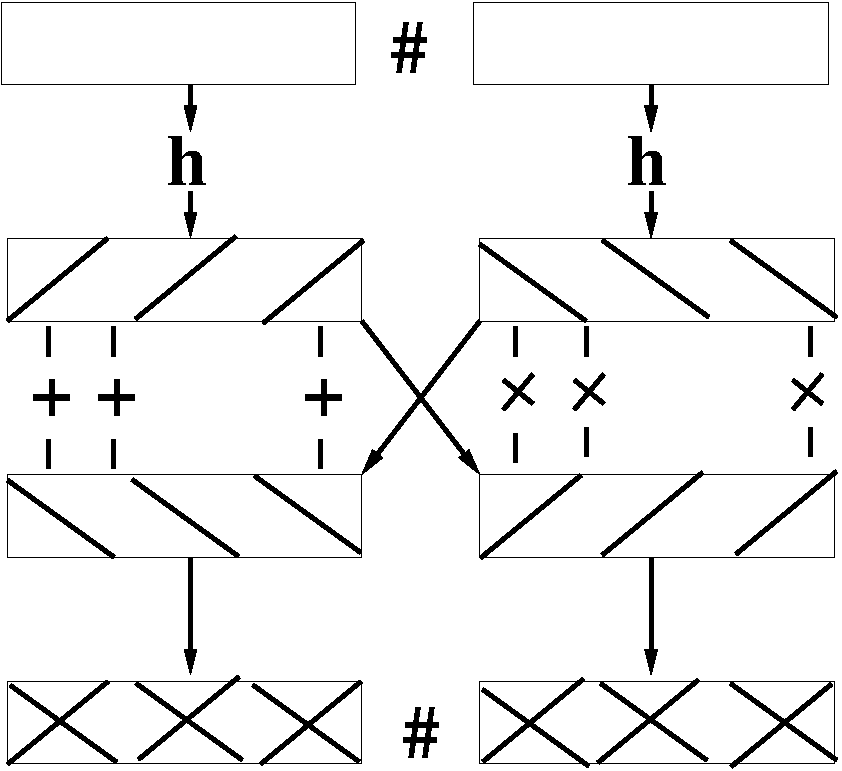
\includegraphics[height=25ex]{Figures/L2/DH}
\column{0.6\textwidth}\vspace{-3ex}
\begin{itemize}
    \item {\tt dhop u v = (zipWith $\oplus$ u v) ++}\\ 
          {\tt~~~~~~~~~~~(zipWith $\otimes$ u v)}
    \item {\tt $\oplus\updownarrow\otimes$ (x ++ y) = ($\oplus\updownarrow\otimes$ x)}\\
          {\tt~~~~~~~~~~`dhop` ($\oplus\updownarrow\otimes$ y)} 
\end{itemize}
\end{columns}

\begin{itemize}
    \item For example, distributed reduction: 
        {\tt distrRed ($\odot$) e$_\odot$ x = }\\
        {\tt [reduce $\odot$ e$_{\odot}$ x,$\ldots$, reduce $\odot$ e$_{\odot}$ x]}
    \item is a DH: distrRed $\odot$ = $\odot\updownarrow\odot$
\end{itemize}

\end{frame}


\begin{frame}[fragile,t]
  \frametitle{Scan is a DH}

\begin{columns}
\column{0.4\textwidth}
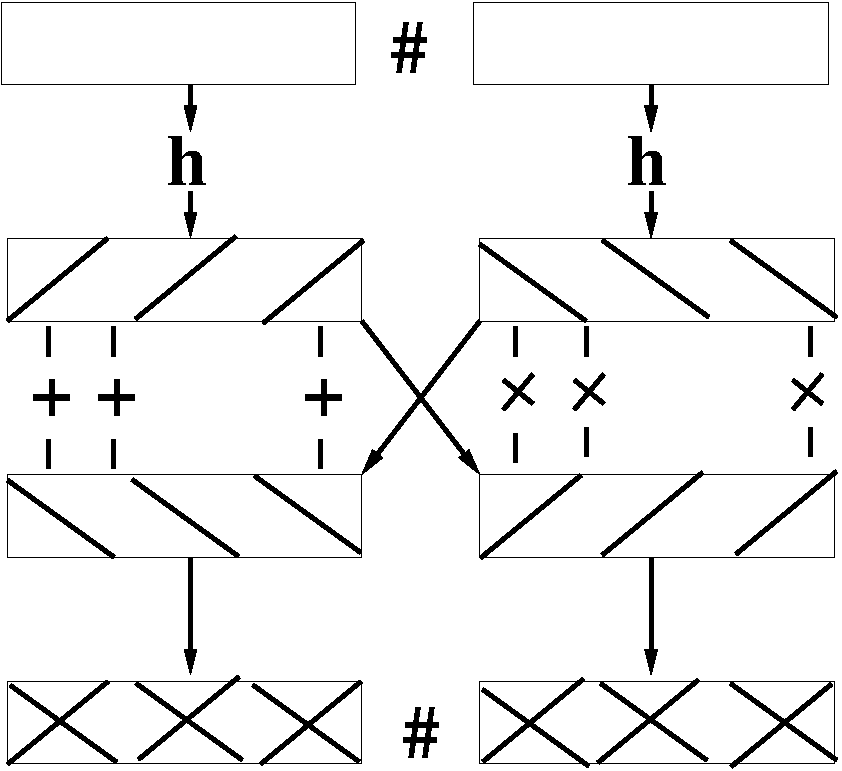
\includegraphics[height=25ex]{Figures/L2/DH}
\column{0.6\textwidth}\vspace{-3ex}
\begin{itemize}
    \item {\tt dhop u v = (zipWith $\oplus$ u v) ++}\\ 
          {\tt~~~~~~~~~~~(zipWith $\otimes$ u v)}
    \item {\tt $\oplus\updownarrow\otimes$ (x ++ y) = ($\oplus\updownarrow\otimes$ x)}\\
          {\tt~~~~~~~~~~`dhop` ($\oplus\updownarrow\otimes$ y)} 
    \item \alert{This implementation of scan is not work efficient,
                i.e., work $O(N \ lg \ N)$!}
\end{itemize}
\end{columns}


\begin{itemize}
    \item ${\tt scan} \ \odot \ {\tt e}_{\odot} \ {\tt(x++y)} = S_1~\oslash~S_2~=~S_1$
            {\tt ++ (map ($\odot$ s) $S_2$)},\\ 
            where $S_1${\tt = scan $\odot$ e$_{\odot}$ x},
                  $S_2${\tt = scan $\odot$ e$_{\odot}$ y}, and {\tt s=last $S_1$}\medskip
 
    \item {\tt dhScan $\odot$ e$_{\odot}$ = (map $\pi_1$) . ($\oplus\updownarrow\otimes$) . (map pair)},\\
            where {\tt $\pi_1$ (a,b) = a,~~~~pair a = (a,a)},\\
            {\tt (s$_1$,r$_1$) $\oplus$ (s$_2$,r$_2$) = (\alert{?}, \alert{?})}\\
            {\tt (s$_1$,r$_1$) $\otimes$ (s$_2$,r$_2$) = (\alert{?}, \alert{?})}
\end{itemize}

\end{frame}


\begin{frame}[fragile,t]
  \frametitle{Scan is a DH}

\begin{columns}
\column{0.4\textwidth}
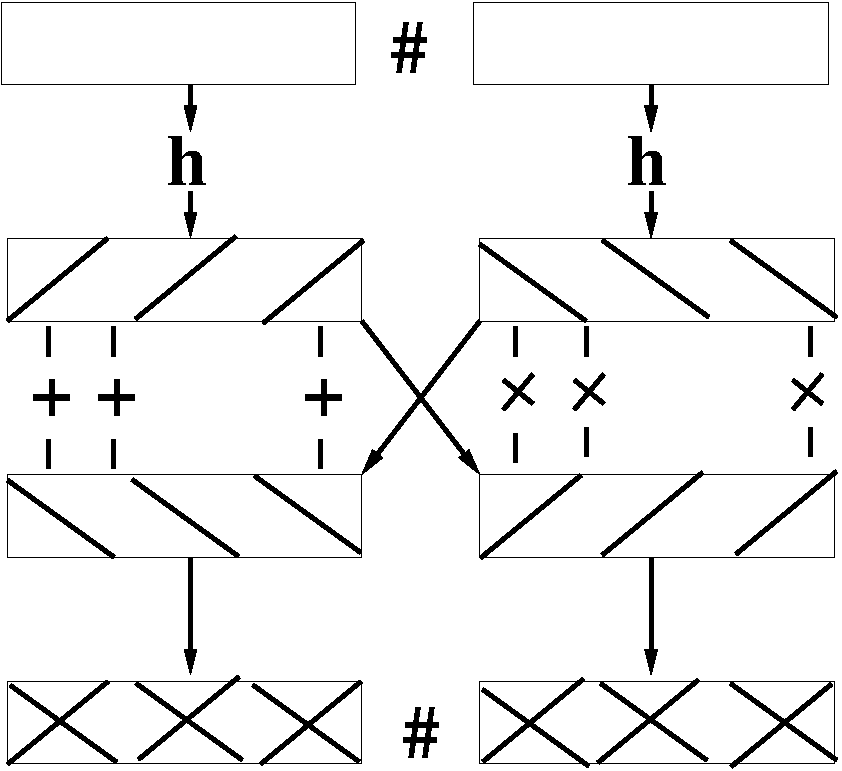
\includegraphics[height=25ex]{Figures/L2/DH}
\column{0.6\textwidth}\vspace{-3ex}
\begin{itemize}
    \item {\tt dhop u v = (zipWith $\oplus$ u v) ++}\\ 
          {\tt~~~~~~~~~~~(zipWith $\otimes$ u v)}
    \item {\tt $\oplus\updownarrow\otimes$ (x ++ y) = ($\oplus\updownarrow\otimes$ x)}\\
          {\tt~~~~~~~~~~`dhop` ($\oplus\updownarrow\otimes$ y)} 
    \item \alert{This implementation of scan is not work efficient,
                i.e., work $O(N \ lg \ N)$!}
\end{itemize}
\end{columns}


\begin{itemize}
    \item ${\tt scan} \ \odot \ {\tt e}_{\odot} \ {\tt(x++y)} = S_1~\oslash~S_2~=~S_1$
            {\tt ++ (map ($\odot$ s) $S_2$)},\\ 
            where $S_1${\tt = scan $\odot$ e$_{\odot}$ x},
                  $S_2${\tt = scan $\odot$ e$_{\odot}$ y}, and {\tt s=last $S_1$}\medskip
 
    \item {\tt dhScan $\odot$ e$_{\odot}$ = (map $\pi_1$) . ($\oplus\updownarrow\otimes$) . (map pair)},\\
            where {\tt $\pi_1$ (a,b) = a,~~~~pair a = (a,a)},\\
            {\tt (s$_1$,r$_1$) $\oplus$ (s$_2$,r$_2$) = (s$_1$, r$_1$ $\odot$ r$_2$)}\\
            {\tt (s$_1$,r$_1$) $\otimes$ (s$_2$,r$_2$) = (r$_1$ $\odot$ s$_2$, r$_1$ $\odot$ r$_2$)}
\end{itemize}

\end{frame}

%%%%%%%%%%%%%%%%%%%%%%%%%%%%%%%%%%%%%%%
%%%%%%%%%%%%%%%%%%%%%%%%%%%%%%%%%%%%%%%
%%%%%%%%%%%%%%%%%%%%%%%%%%%%%%%%%%%%%%%
\section{Implementation of Flat Bulk Operators}

\begin{frame}[fragile]
	\tableofcontents[currentsection]
\end{frame}

\subsection{Implementation of Reduce and Scan}

\begin{frame}[fragile,t]
  \frametitle{Map, Reduce, and Scan Types and Semantics}

\begin{itemize}
    \item \emp{\tt map~::~($\alpha\rightarrow\beta$)~$\rightarrow$~[$\alpha$]$~\rightarrow$~[$\beta$]}\\
    \emph{\tt map f [x$_1,\ldots, $x$_n$] = [f(x$_1$),$\ldots$, f(x$_n$)]},\\  
        i.e., \emp{\tt{}x$_i$~::~$\alpha, \forall i$}, and 
        \emp{\tt f~::~$\alpha\rightarrow\beta$}.\medskip

    \item \emp{{\tt reduce~::~($\alpha$~$\rightarrow$~$\alpha$~$\rightarrow$~$\alpha$)~$\rightarrow$~$\alpha$~$\rightarrow$~[$\alpha$]~$\rightarrow$~$\alpha$}}\\
        \emph{\tt reduce $\odot$~e~[x$_1$,x$_2$,..,x$_n$]~=~e$\odot$x$_1\odot$x$_2\odot\ldots\odot$x$_n$},\\
        i.e., \emp{{\tt{}e::$\alpha$, x$_i$~::~$\alpha, \forall i$}}, and 
        \emp{\tt $\odot$~::~$\alpha\rightarrow\alpha\rightarrow\alpha$}.\medskip

    \item \emp{{\tt scan$^{exc}$~::~($\alpha$~$\rightarrow$~$\alpha$~$\rightarrow$~$\alpha$)~$\rightarrow$~$\alpha$~$\rightarrow$~[$\alpha$]~$\rightarrow$~[$\alpha$]}}\\
        \emph{\tt scan$^{exc}~\odot$~e~[x$_1$,$\ldots$,x$_n$]~=~[e,e$\odot$x$_1$,$\ldots$,e$\odot$x$_1\odot\ldots$x$_{n-1}$]}\\
        i.e., \emp{{\tt{}e::$\alpha$, x$_i$~::~$\alpha, \forall i$}}, and 
        \emp{\tt $\odot$~::~$\alpha\rightarrow\alpha\rightarrow\alpha$}.\medskip

    \item \emp{{\tt scan$^{inc}$~::~($\alpha$~$\rightarrow$~$\alpha$~$\rightarrow$~$\alpha$)~$\rightarrow$~$\alpha$~$\rightarrow$~[$\alpha$]~$\rightarrow$~[$\alpha$]}}\\
        \emph{\tt scan$^{inc}~\odot$~e~[x$_1$,$\ldots$,x$_n$]~=~[e$\odot$x$_1$,$\ldots$,e$\odot$x$_1\odot\ldots$x$_{n}$]}\\
        i.e., \emp{{\tt{}e::$\alpha$, x$_i$~::~$\alpha, \forall i$}}, and 
        \emp{\tt $\odot$~::~$\alpha\rightarrow\alpha\rightarrow\alpha$}.

\end{itemize}

\end{frame}

\begin{frame}[fragile,t]
  \frametitle{Parallel Random Access Machine (PRAM)}

PRAM focuses exclusively on parallelism and ignores issues
related to synchronization and communication:
\begin{itemize}
    \item[1] $p$ processors connected to shared memory
    \item[2] each processor has an unique id (index) $i$, $1 \leq i \leq p$
    \item[3] SIMD execution, each parallel instruction requires unit time,
    \item[4] each processor has a flag that controls whether it is active
                in the execution of an instruction.
\end  {itemize}

\pause

\begin{columns}
\column{0.5\textwidth}
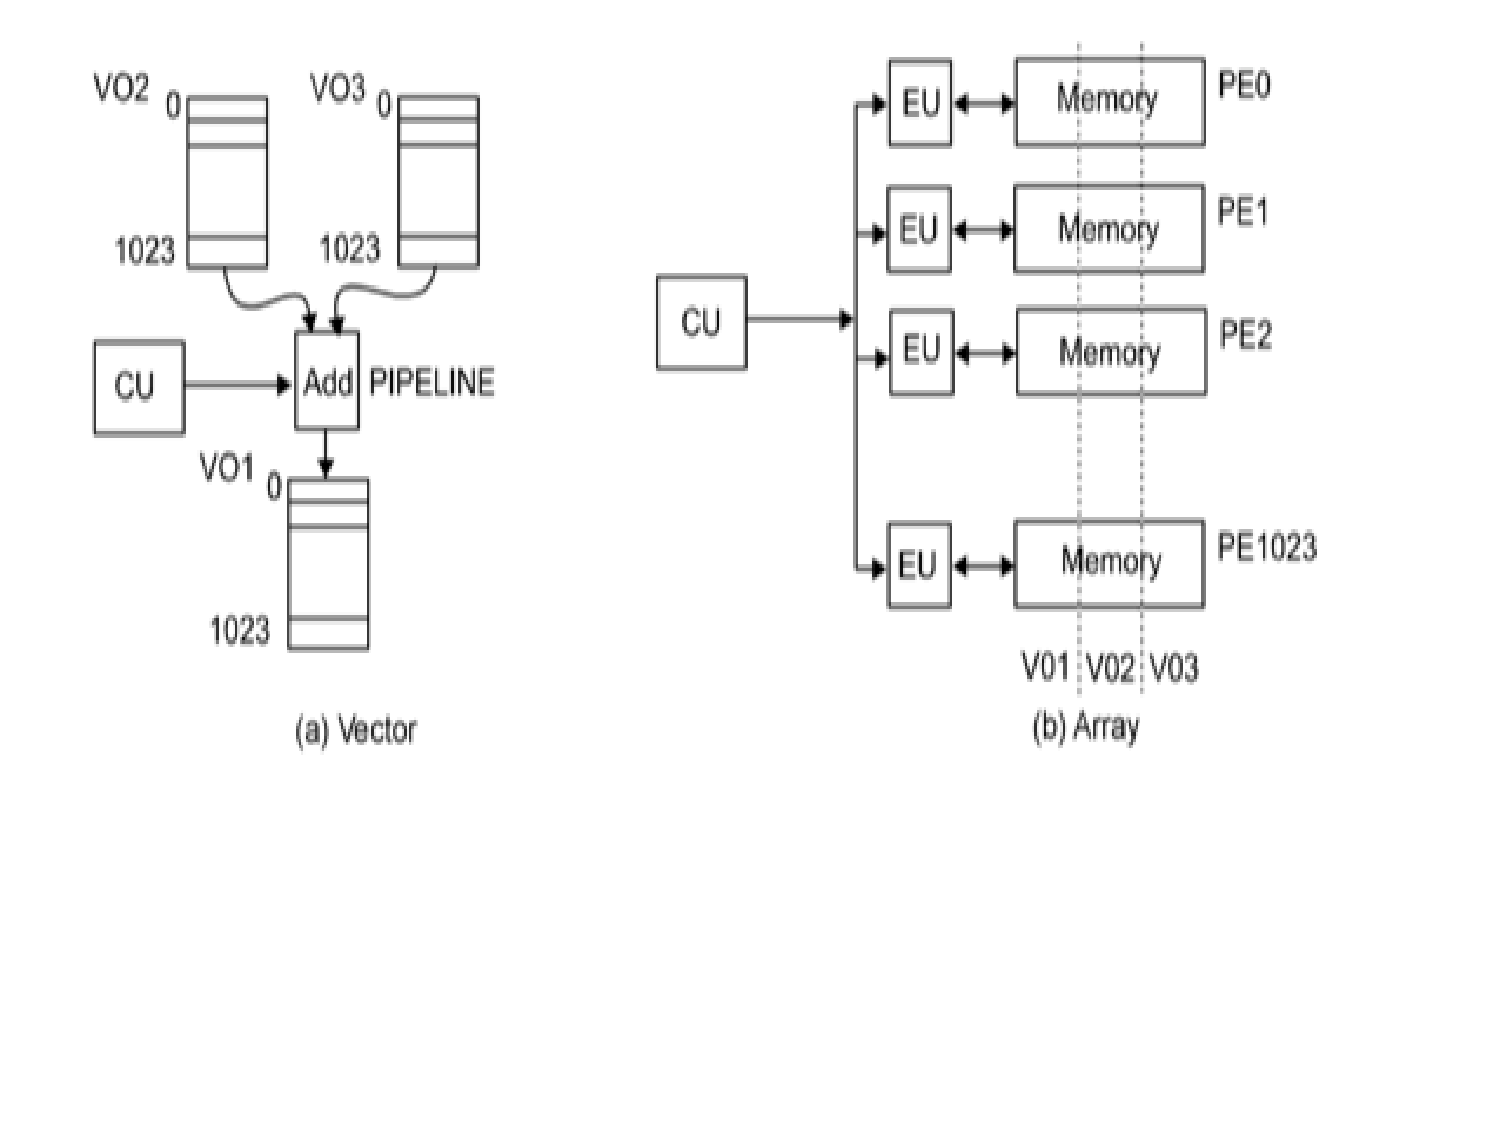
\includegraphics[height=33ex]{Figures/L2/VectorMachine}
\column{0.55\textwidth}\vspace{-15ex}
\begin{itemize}
    \item \emp{Work Time Algorithm (WT):}
    \begin{itemize}
        \item \emp{Work Complexity W(n)}:       is the total \# of ops performed,
        \item \emp{Depth/Step Complexity D(n)}: is the \# of sequential steps.
    \end{itemize}
    \item If we know WT's work and depth, then Brent Theorem 
            gives good complexity bounds for a PRAM.
\end{itemize}
\end{columns}

\end{frame}


\begin{frame}
  \frametitle{Reducing in Parallel}

\begin{columns}
\column{0.6\textwidth}
        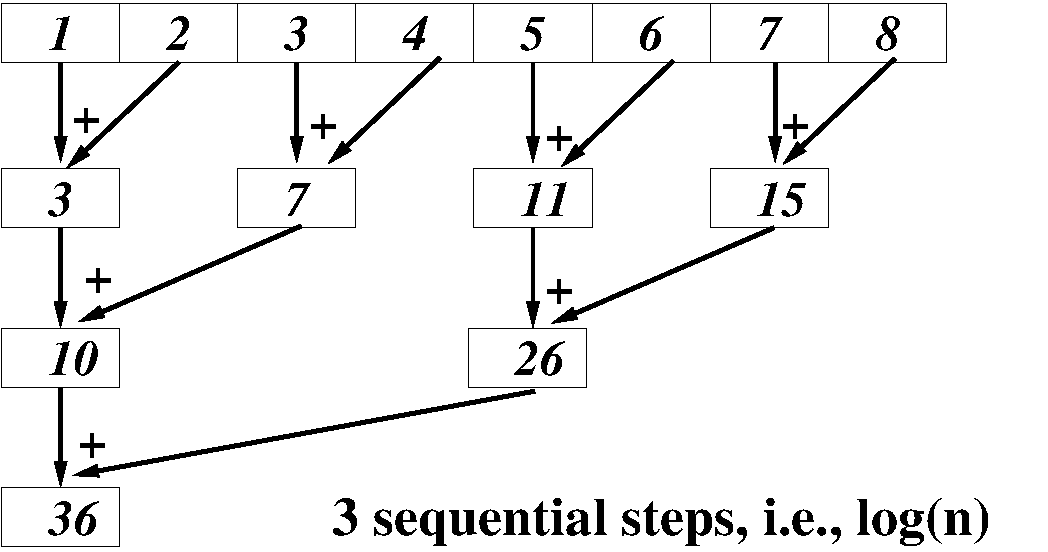
\includegraphics[height=22ex]{Figures/L2/ReduceEg.pdf} 
\column{0.5\textwidth}
Reducing an array of length {\tt n} with {\tt  n/2} processors requires:
\begin{itemize}
    \item work $W(n) = n$ and 
    \item depth $D(n) = lg \ n$, i.e., number of sequential steps.
    \item optimized runtime with $P$ processors: \emph{$(n/P) + lg \ P$.}
\end  {itemize}
\end{columns}

\begin{mytheo}[Brent Theorem]\label{BrentTh}
A Work-Time Algorithm of depth $D(n)$ and work $W(n)$ can be
simulated on a $P$-processor PRAM in time complexity T such that:\\\bigskip
\emp{$\ \ \ \ \ \ \ \ \ \ \ \ \ \ \ \ \frac{W(n)}{P} \leq T < \frac{W(n)}{P} + D(n)$}
\end{mytheo}

\end{frame}


\begin{frame}[fragile,t]
  \frametitle{Reduce: Algorithm and Complexity}


\begin{columns}
\column{0.5\textwidth}
\begin{colorcode}[fontsize=\scriptsize]
Input:  array A of n=2\mymath{\myindu{k}} elems of type T
        \mymath{\oplus::T\times T\rightarrow T} associative
Output: S = \mymath{\oplus\myindx{j=1}\myindu{n} a\myindx{j}}

1.  \emph{forall i = 0 to n-1 do}
2.    B[i] \mymath{\leftarrow} A[i]
3.  \emph{enddo}

4.  \emp{for h = 1 to k do}
5.    \emph{forall i = 0 to n-1 by 2\mymath{\myindu{h}} do} 
6.      B[i] \mymath{\leftarrow} B[i] \mymath{\oplus} B[i+2\mymath{\myindu{h-1}}]
7.    \emph{enddo}
8.  \emp{enddo}
9.  S \mymath{\leftarrow} B[0]  
\end{colorcode}
\column{0.59\textwidth}
\begin{itemize}
    \item $D_{1-3}(n) = \Theta(1)$, $W_{1-3}(n) = \Theta(n)$,
    \item $D_{5-7}(n) = \Theta(1)$, $W_{5-7}(n,h) = \Theta(n/2^h)$,
    \item $D_{4-8}(n) = k \times D_{5-7}(n) = \Theta(lg \ n)$
    \item $W_{4-8}(n) = \sum_{h=1}^k W_{5-7}(n,h) = $\\
          $\Theta(\sum_{h=1}^k (n/2^h) ) = \Theta(n)$
    \item $D_{9}(n) = \Theta(1)$, $W_{9}(n) = \Theta(1)$,\bigskip
    \item \emp{$D(n) = \Theta(lg \ n), W(n) = \Theta(n)$!}
\end{itemize}
\end{columns}
\bigskip

%\mymath{\frac{n}{2\myindu{h}}} do}

\begin{center}  
\emp{$\frac{n-1}{P} \leq  Runtime < \frac{n-1}{P} + lg \ n$}
\end{center}


\end{frame}


\begin{frame}[fragile,t]
  \frametitle{Parallel Exclusive Scan with Associative Operator $\oplus$}
\bigskip

\begin{columns}
\column{0.4\textwidth}
        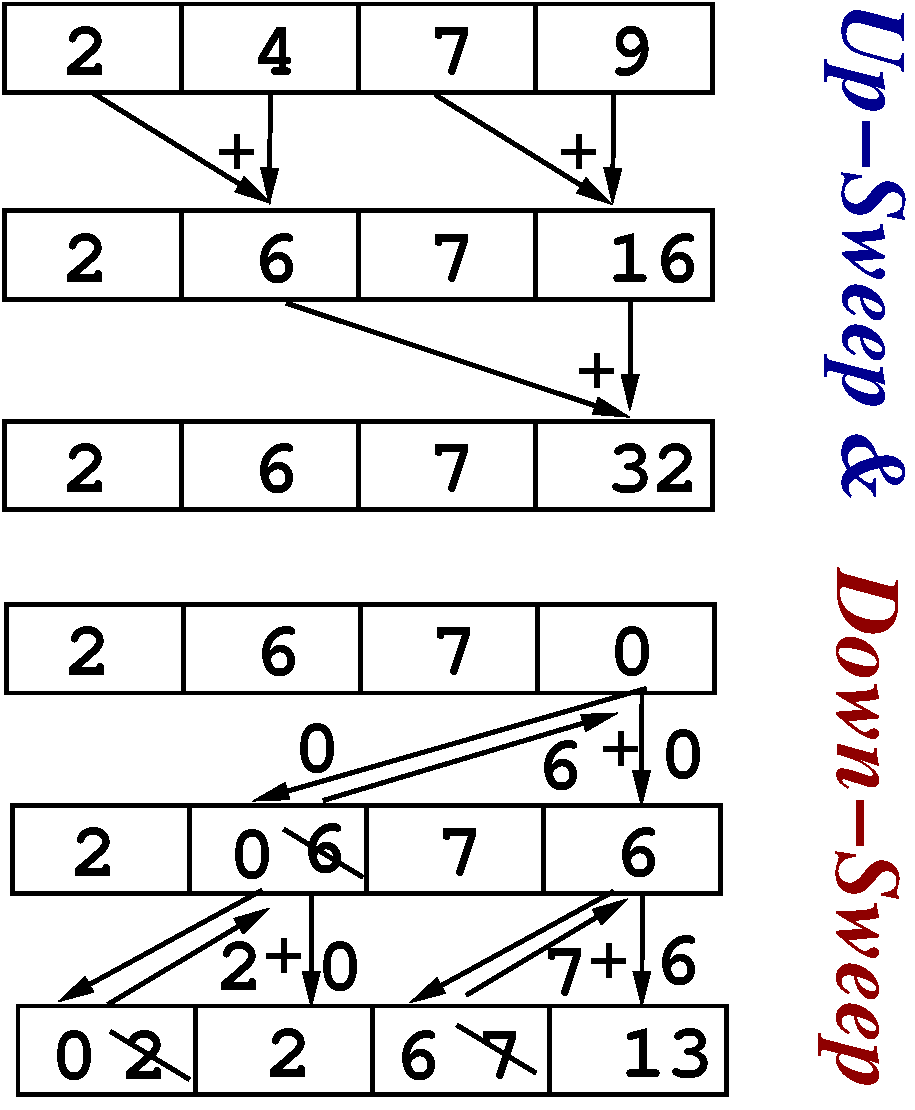
\includegraphics[height=33ex]{Figures/L2/ScanEg.pdf} 
\column{0.6\textwidth}
Two Steps:
\begin{itemize}
    \item \blue{Up-Sweep:} similar with reduction
    \item Root is replaced with neutral element.
    \item \emp{Down-Sweep:} 
    \begin{itemize}
        \item the left child sends its value to parent and 
                updates its value to that of parent.
        \item the right-child value is given by $\oplus$ 
                applied to the left-child value and
                the (old) value of parent.
        \item note that the right child is in fact the parent,
                i.e., in-place algorithm.
    \end  {itemize}
\end  {itemize}
\end{columns}


\end{frame}



\begin{frame}[fragile,t]
  \frametitle{Parallel Exclusive Scan Algorithm And Complexity}
\bigskip

\begin{columns}
\column{0.5\textwidth}
\begin{colorcode}[fontsize=\scriptsize]
Input:  array A of n=2\mymath{\myindu{k}} elems of type T
        \mymath{\oplus::T\times T\rightarrow T} associative
Output: B = \mymath{[0, a\myindx{1}, a\myindx{1}\oplus{}a\myindx{2},\ldots,\oplus\myindx{j=1}\myindu{n-1} a\myindx{j}]}

1.  \emph{forall i = 0 : n-1 do}
2.    B[i] \mymath{\leftarrow} A[i]
3.  \emph{enddo}

4.  \emp{for d = 0 to k-1 do} \emph{// up-sweep}
5.    \emph{forall i = 0 to n-1 by 2\mymath{\myindu{d+1}} do} 
6.      B[i+2\mymath{\myindu{d+1}}-1] \mymath{\leftarrow} B[i+2\mymath{\myindu{d}}  -1] \mymath{\oplus} 
                       B[i+2\mymath{\myindu{d+1}}-1]
7.    \emph{enddo}
8.  \emp{enddo}
9.  B[n-1] = 0
10. \emp{for d = k-1 downto 0 do} \emph{// down-sweep}
11.   \emph{forall i = 0 to n-1 by 2\mymath{\myindu{d+1}} do} 
12.     tmp \mymath{\leftarrow} B[i+2\mymath{\myindu{d}}-1]
13.     B[i+2\mymath{\myindu{d}}-1] \mymath{\leftarrow} B[i+2\mymath{\myindu{d+1}}-1]
14.     B[i+2\mymath{\myindu{d+1}}-1] \mymath{\leftarrow} tmp \mymath{\oplus} B[i+2\mymath{\myindu{d+1}}-1]
15.   \emph{enddo}
16. \emp{enddo}
\end{colorcode}
\column{0.59\textwidth}
\begin{itemize} 
    \item The code show exponentials for clarity, but those can
            be computed by one multiplication/division operation
            each sequential iteration.
    \item \emp{$D(n) = \Theta(lg \ n), W(n) = \Theta(n)$!}
    \item Similar reasoning as with reduce.
\end{itemize}
\end{columns}

%4.  \emp{for h = 1 to k do} // up-sweep
%5.    \emph{forall i \mymath{\in} n : 1 by -2\mymath{\myindu{h}} do} 
%6.      B[i] \mymath{\leftarrow} B[i] \mymath{\oplus} B[i-2\mymath{\myindu{h-1}}]
%7.    \emph{enddo}
%8.  \emp{enddo}
%9.  B[n] = 0
%
%10. \emp{for h = k downto 1 do} // down-sweep
%11.   \emph{forall i \mymath{\in} n : 1 by -2\mymath{\myindu{h}} do} 
%12.     tmp = B[i]
%13.     B[i] \mymath{\leftarrow} B[i] \mymath{\oplus} B[i-2\mymath{\myindu{h-1}}]
%14.     B[i-2\mymath{\myindu{h-1}}] = tmp
%15.   \emph{enddo}
%16. \emp{enddo}


\end{frame}

%%%%%%%%%%%%%%%%%%%%%%%%%%%%%%%%%%%%%%%%%
%%%%%%%%%%%%%%%%%%%%%%%%%%%%%%%%%%%%%%%%%
\subsection{Other Second-Order Bulk Operators}

\begin{frame}[fragile,t]
  \frametitle{Zip, ZipWith}

\begin{itemize}
    \item \emph{\tt zip :: [$\alpha_1$] $\rightarrow$ [$\alpha_2$] $\rightarrow$ [($\alpha_1$,$\alpha_2$)]}
    \item \emp{\tt zip [a$_1$,$\ldots$,a$_n$] [b$_1$,$\ldots$,b$_m$] $\equiv$ [(a$_1$,b$_1$),\ldots,(a$_q$,b$_q$)]},
            where {\tt q = min(m,n)}.\pause
    \item \emph{\tt unzip :: [($\alpha_1$,$\alpha_2$)] $\rightarrow$ ([$\alpha_1$],[$\alpha_2$])}
    \item \emp{\tt unzip [(a$_1$,b$_1$),\ldots,(a$_n$,b$_n$)]$\equiv$([a$_1$,$\ldots$,a$_n$],[b$_1$,$\ldots$,b$_n$])},\pause\medskip

    \item In some sense {\tt zip} is syntactic sugar, for example one could work with the
            tuple of array representation, e.g.,
    \item \emp{\tt mapT :: (($\alpha_1$,$\ldots$,$\alpha_m$)$\rightarrow$($\beta_1$,$\ldots$,$\beta_n$)) $\rightarrow$}\\ 
          \emp{\tt~~~~~~~~~[$\alpha_1$] $\rightarrow\ldots\rightarrow$ [$\alpha_m$] $\rightarrow$ ([$\beta_1$],$\ldots$,[$\beta_n$]])}
    \item \emph{\tt mapT f $\equiv$ unzip$^n$ . map f . zip$^n$}\pause\medskip

    \item {\tt zipWith :: ($\alpha_1\rightarrow\alpha_2\rightarrow\beta$) $\rightarrow$ [$\alpha_1$] $\rightarrow$ [$\alpha_2$] $\rightarrow$ [$\beta$]}
    \item {\tt zipWith $\odot$ [a$_1$,$\ldots$,a$_n$] [b$_1$,$\ldots$,b$_n$] $\equiv$ [a$_1\odot$b$_1$,$\ldots$,a$_n\odot$b$_n$]}
    \item {\tt zipWith $\odot$ $\equiv$ map ($\backslash$(u,v) $\rightarrow$ u $\odot$ v) . zip}
\end  {itemize}

\end{frame}

\begin{frame}[fragile,t]
  \frametitle{Permute, Write, Split, Filter}

\begin{itemize}
    \item Operator to \emph{write in parallel} a set of values to 
            correspond indices:\\
          \emph{write :: [Int] $\rightarrow$ [$\alpha$] $\rightarrow$ [$\alpha$] $\rightarrow$ [$\alpha$]}\\
          A (data vector) {\tt~=[b0, b1, b2]}\\
          I (index vector){\tt~~=[2,~~4,~~1]}\\
          X (input array) {\tt~=[a0,~a1,~a2,~a3,~a4,~a5]}\\
          \emp{write I A X     {\tt~~~~=[a0,~b2,~b0,~a3,~b1,~a5]}}\bigskip

    \item Operator to \emph{permute in parallel} based on a set (array) of indices:\\
          \emph{permute::[Int]$\rightarrow$[$\alpha$]$\rightarrow$[$\alpha$]}. {\small~\blue{\tt permute~I~A~$\equiv$~write~I~A~(copy~A)}}\\
           A (data vector) {\tt~= [a0,~a1,~a2,~a3,~a4,~a5]}\\
           I (index vector){\tt~~= [3,~~2,~~0,~~4,~~1,~~5~]}\\
           \emp{permute I A     {\tt~~~~= [a2,~a4,~a1,~a0,~a3,~a5]}}\\\bigskip
           

    \item %Operator to {\tt split} a list (array) at a certain index:\\
          \emph{\tt split :: Int $\rightarrow$ [$\alpha$] $\rightarrow$ ([$\alpha$],[$\alpha$])}\\
          \emp{\tt split i [a$_0$,$\ldots$,a$_n$] $\equiv$ ([a$_0$,$\ldots$,a$_{i-1}$], [a$_i$,$\ldots$,a$_{n}$])}\smallskip
    \item \emph{\tt replicate :: Int $\rightarrow$ $\alpha$ $\rightarrow$ [$\alpha$]}\\
            \emp{\tt replicate N a $\equiv$ [a, a,$\ldots$, a]}, i.e., {\tt a} is replicated {\tt N} times.  
 
\end  {itemize}

\end{frame}

\begin{frame}[fragile,t]
  \frametitle{Filter: Implementation based on Map and Scan}

%\mymath{\backslash}

\emph{\tt filter :: ($\alpha\rightarrow$Bool) $\rightarrow$ [$\alpha$] $\rightarrow$ [$\alpha$]}\\
Filters out the input-list elements that do NOT satisfy the predicate.
%\emp{\tt filter cond X $\equiv$ [b$_0$,$\ldots$,b$_{m}$]}, such that 
%{\tt b$_j, \forall j\in\{0\ldots m\}$,} are all the elements of array 
%{\tt X} that evaluate to {\tt True} under condition {\tt cond}, i.e., {\tt (cond b$_j$) $\equiv$ True}.\medskip

\alert{Can {\tt filter} be implemented via {\tt map} and {\tt reduce} (and {\tt scan})?}\pause


\begin{columns}
\column{0.59\textwidth}
\begin{colorcode}[fontsize=\scriptsize]
parFilter :: (a->Bool) -> [a] -> ([a], [Int])
parFilter cond X = 
let n   = length arr
    cs  = map cond X
    tfs = map (\mymath{\backslash}f->if f then 1 
                        else 0) cs
    isT = scan\mymath{\myindu{inc}} (+) 0 tfs
    i   = last isT

    ffs = map (\mymath{\backslash}f->if f then 0 
                        else 1) cs
    isF = (map (+ i) . scan\mymath{\myindu{inc}} (+) 0) ffs

    inds= map (\mymath{\backslash} (c,iT,iF) -> 
                  if c then iT-1 else iF-1 ) 
              (zip3 cs isT isF)
    flags = write [0,i] [i,n-i] (replicate n 0)
in  (permute X inds, flags)
\end{colorcode}
\column{0.4\textwidth}
\begin{colorcode}[fontsize=\scriptsize]
Assume X = [5,4,2,3,7,8], and 
cond is T(rue) for even nums.
n   = 6
cs  = [F, T, T, F, F, T]
tfs = [0, 1, 1, 0, 0, 1]

isT = [0, 1, 2, 2, 2, 3]
i   = 3

ffs = [1, 0, 0, 1, 1, 0]

isF = [4, 4, 4, 5, 6, 6]

inds= [3, 0, 1, 4, 5, 2]


flags  = [3, 0, 0, 3, 0, 0]
Result = [4, 2, 8, 5, 3, 7] 
\end{colorcode}
\end{columns}

\end{frame}

\subsection{Implementation of Segmented Scan}

\begin{frame}[fragile]
	\tableofcontents[currentsubsection]
\end{frame}


\begin{frame}[fragile,t]
  \frametitle{Segmented Inclusive Scan with Operator $\oplus$}

\emphh{Equiv with Mapping a Scan op on each segment of an irregular array.}

\begin{columns}
\column{0.55\textwidth}
\begin{colorcode}
-- iota n = [0..n-1]
map (\mymath{\backslash}i-> scan (+) 0 [1..i]) [3,4] \emph{\mymath{\equiv}}
[ scan\mymath{\myindu{inc}} (+) 0 [1,2,3], 
  scan\mymath{\myindu{inc}} (+) 0 [1,2,3,4] ] 
      \emph{\mymath{\equiv}}
[ [1,3,6], [1,3,6,10] ]
\end{colorcode}
\column{0.55\textwidth}
\begin{colorcode}
-- \blue{Flags \& Flat Data Representation:}
sgmScanInc (+) 0 [1,0,0,1,0,0,0] -- \emph{flag}
                 [1,2,3,1,2,3,4] -- \emp{data}
    \emph{\mymath{\equiv}}
( [1,0,0,1,0,0, 0],              -- \emph{flag}
  [1,3,6,1,3,6,10] )             -- \emp{data}
\end{colorcode}
\end{columns}
\medskip

\emphh{Can be obtained by replacing the following operator:}
\smallskip

\begin{colorcode}
sgmScanInc :: (a->a->a) -> a -> [Int] -> [a] -> [a]
sgmScanInc \mymath{\odot} ne flags data = 
  let fds = zip flags data
      (_,r) = unzip \$ 
              scan\mymath{\myindu{inc}} (\mymath{\backslash}(f1,v1) (f2,v2) -> 
                        let f = f1 .|. f2  -- bitwise or
                        in  if f2 == 0
                            then (f, v1 \mymath{\odot} v2)
                            else (f, v2)
                     ) (0,ne) fvs
  in  r
\end{colorcode}
\bigskip

\alert{How about Exclusive Scan?}

\end{frame}

\begin{frame}[fragile,t]
  \frametitle{{\scriptsize Slide from CMU 15-418: Parallel Computer Architecture and Programming (Spring 2012)}}
\vspace{-3ex}
\begin{center}
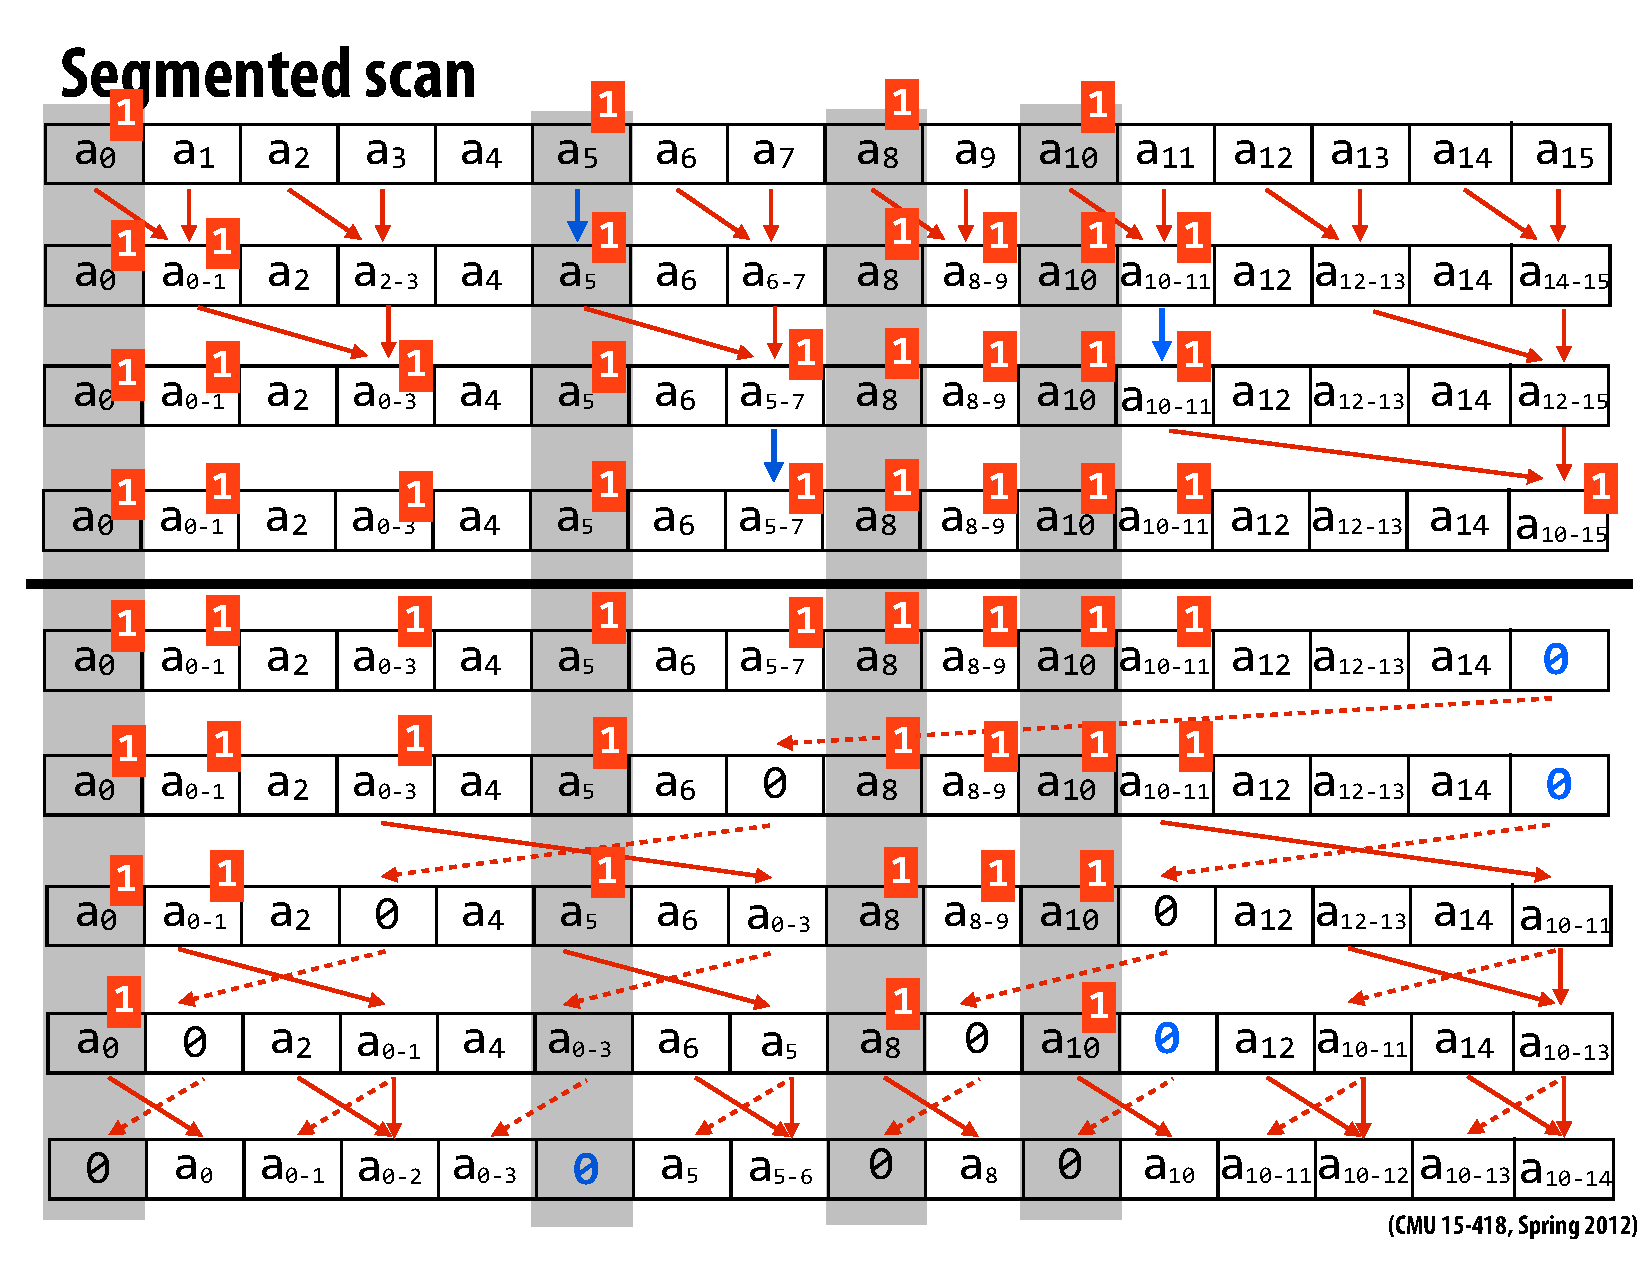
\includegraphics[height=50ex]{Figures/L2/SegmExclScan} 
\end  {center}

\end{frame}


\begin{frame}[fragile,t]
  \frametitle{Segmented Exclusive Scan Alg And Complexity}
\vspace{-2ex}
\begin{columns}
\column{0.6\textwidth}
\begin{colorcode}[fontsize=\scriptsize]
Input:  flag array F of n=2\mymath{\myindu{k}} of ints
        data array A of n=2\mymath{\myindu{k}} elems of type T
        \mymath{\oplus::T\times T\rightarrow T} associative
Output: B = segmented scan of 2-dim array A
1.  \emph{FORALL i = 0 to n-1 do} B[i] \mymath{\leftarrow} A[i] \emph{ENDDO}
2.  \emp{FOR d = 0 to k-1 DO} \emph{// up-sweep}
3.    \emph{FORALL i = 0 to n-1 by 2\mymath{\myindu{d+1}} DO} 
4.      IF F[i+2\mymath{\myindu{d+1}}-1] == 0 THEN 
5.          B[i+2\mymath{\myindu{d+1}}-1] \mymath{\leftarrow} B[i+2\mymath{\myindu{d}}-1] \mymath{\oplus} B[i+2\mymath{\myindu{d+1}}-1]
6.      ENDIF
7.      F[i+2\mymath{\myindu{d+1}}-1] \mymath{\leftarrow} F[i+2\mymath{\myindu{d}}-1] .|. F[i+2\mymath{\myindu{d+1}}-1]
8.  \emp{ENDDO} \emph{ENDDO}
9.  B[n-1] \mymath{\leftarrow} 0
10. \emp{FOR d = k-1 downto 0 DO} \emph{// down-sweep}
11.   \emph{FORALL i = 0 to n-1 by 2\mymath{\myindu{d+1}} DO} 
12.     tmp \mymath{\leftarrow} B[i+2\mymath{\myindu{d}}-1]
13.     IF \alert{F\_original}[i+2\mymath{\myindu{d}}] \mymath{\neq} 0 THEN
14.          B[i+2\mymath{\myindu{d+1}}-1] \mymath{\leftarrow} 0
15.     ELSE IF F[i+2\mymath{\myindu{d}}-1] \mymath{\neq} 0 THEN
16.          B[i+2\mymath{\myindu{d+1}}-1] \mymath{\leftarrow} tmp
17.     ELSE B[i+2\mymath{\myindu{d+1}}-1] \mymath{\leftarrow} tmp \mymath{\oplus} B[i+2\mymath{\myindu{d+1}}-1]
18.     ENDIF
19.     F[i+2\mymath{\myindu{d+1}}-1] \mymath{\leftarrow} 0
20. \emp{ENDDO} \emph{ENDDO}
\end{colorcode}
\column{0.35\textwidth}
\begin{itemize} 
    \item While there are more branches, the asymptotics 
            does not change:
    \item \emph{$D(n) = \Theta(lg \ n)$},\\\emp{$W(n) = \Theta(n)$!}
\end{itemize}
\end{columns}

%4.  \emp{for h = 1 to k do} // up-sweep
%5.    \emph{forall i \mymath{\in} n : 1 by -2\mymath{\myindu{h}} do} 
%6.      B[i] \mymath{\leftarrow} B[i] \mymath{\oplus} B[i-2\mymath{\myindu{h-1}}]
%7.    \emph{enddo}
%8.  \emp{enddo}
%9.  B[n] = 0
%
%10. \emp{for h = k downto 1 do} // down-sweep
%11.   \emph{forall i \mymath{\in} n : 1 by -2\mymath{\myindu{h}} do} 
%12.     tmp = B[i]
%13.     B[i] \mymath{\leftarrow} B[i] \mymath{\oplus} B[i-2\mymath{\myindu{h-1}}]
%14.     B[i-2\mymath{\myindu{h-1}}] = tmp
%15.   \emph{enddo}
%16. \emp{enddo}


\end{frame}


%%%%%%%%%%%%%%%%%%%%%%%%%%%%%%%%%%%%%%%%%%%%%
%%%%%%%%%%%%%%%%%%%%%%%%%%%%%%%%%%%%%%%%%%%%%
%%%%%%%%%%%%%%%%%%%%%%%%%%%%%%%%%%%%%%%%%%%%%


\section{Nested Data-Parallel Applications} 

\begin{frame}[fragile]
	\tableofcontents[currentsection]
\end{frame}

\subsection{Sieve: Prime-Numbers Computation}

\begin{frame}[fragile,t]
  \frametitle{Computing Prime Numbers: First Attempt}

See also "Scan as Primitive Parallel Operation" [Bleelloch]\\
(attached in Additional Teaching Material module).

\medskip

Start with an array of size $n$ filled initially with $1$,
i.e., all are primes, and iteratively zero out all multiples
of numbers up to $\sqrt{n}$.
\bigskip

\begin{colorcode}
int res[n] = \{0, 0, 1, 1, 1, ..., 1\}
for(i = 2; i < sqrt(n); i++) \{  \alert{//sequential}
    if ( res[i] != 0 ) \{
        \emph{forall m \mymath{\in multiples of i \leq n} do} \{
             res[m] = 0;
        \}
    \}
\}
\end{colorcode}
\bigskip

\emph{Work: $O(n \ lg \ lg \ n)$} but \emp{Depth: $O(\sqrt{n})$ (Not Good Enough!)}

\end{frame}

\begin{frame}[fragile,t]
  \frametitle{Computing Prime Numbers: First Attempt}

Start with an array of size $n$ filled intially with $1$,
i.e., all are primes, and iteratively zero out all multiples
of numbers up to $\sqrt{n}$.

\begin{columns}
\column{0.59\textwidth}
\begin{colorcode}[fontsize=\scriptsize]
primes :: Int -> [Int]
primes n = 
  let a = map (\mymath{\backslash}i -> if i==0 || i==1
                     then 0
                     else 1 ) [0..n]
      sqrtN = floor (sqrt (fromIntegral n))
  in  primesHelp 2 n sqrtN a
  where
    primesHelp :: Int -> Int -> Int 
               -> [Int] -> [Int]
    primesHelp i n sqrtN a = 
      if i > sqrtN then a
      else let m    = (n `div` i) - 1
               inds = \emph{map (\mymath{\backslash}k -> (k+2)*i)} 
                          \emph{[0..m-1]} --(iota m)
               vals = \emph{replicate m 0}
               a'   = \emph{write inds vals a}
           in  primesHelp (i+1) n sqrtN a'
\end{colorcode}
\column{0.4\textwidth}
\begin{colorcode}[fontsize=\scriptsize]
Assume n = 9, sqrtN = 3 
a = [0,0,1,1,1,1,1,1,1,1]

call primesHelp 2 a
m    = (9 `div` 2) - 1 = 3
inds = [4, 6, 8]
vals = [0, 0, 0]
a' = [0,0,1,1,\emp{0},1,\emp{0},1,\emp{0},1]

call primesHelp 3 a'
m    = (9 `div` 3) - 1 = 2
inds = [6, 9]
vals = [0, 0]
a''= [0,0,1,1,0,1,\emp{0},1,0,\emp{0}]

call primesHelp 4 a''
result: [0,0,\emp{1},\emp{1},0,\emp{1},0,\emp{1},0,\emp{0}]
  i.e., [0,1,\emp{2},\emp{3},4,\emp{5},6,\emp{7},8,9]
\end{colorcode}
\end{columns}
\medskip

\emph{Work: $O(n \ lg \ lg \ n)$} but \emp{Depth: $O(\sqrt{n})$ (Not Good Enough!)}

\end{frame}


\begin{frame}[fragile,t]
  \frametitle{Computing Prime Numbers: Nested Parallelism}
\vspace{-2ex}
If we have all primes from $2$ to $\sqrt{n}$ we could
generate all multiples of these primes at once:
\emp{\tt \{[2*p:n:p]: p in sqr\_primes\}} in NESL.
\blue{Also call algorithm recursively on $\sqrt{n}$ $\Rightarrow$ Depth: $O(lg \ lg \ n)$!}\\
(solution of $n^{(1/2)^{depth}}=2$).
\pause
\begin{columns}
\column{0.59\textwidth}
\begin{colorcode}[fontsize=\scriptsize]
primesOpt :: Int -> [Int]
primesOpt n = 
  if n <= 2 then [2]
  else 
   let sqrtN = floor (sqrt (fromIntegral n))
       \blue{sqrt_primes = primesOpt sqrtN}
       nested = \emp{map} (\mymath{\backslash}\emp{p}->let m = (n `div` p) 
                         in  \emp{map} (\mymath{\backslash}j-> j*p)
                                 [2..m]
                    ) \emp{sqrt_primes}
       not_primes  = \emph{reduce} (++) [] nested
       mm = length not_primes
       zeros = \emph{replicate} mm False 
       prime_flags= \emph{write} not_primes zeros 
                    \emph{(replicate} (n+1) True)
       (primes,_)= unzip $ \emph{filter} (\mymath{\backslash}(i,f)->f) 
                    $ (zip [0..n] prime_flags)
   in drop 2 primes
\end{colorcode}
\column{0.4\textwidth}\pause
\begin{colorcode}[fontsize=\scriptsize]
Assume n = 9, sqrtN = 3 

call primesOpt 3
n = 3,sqrtN = 1,sqrt_primes=[2]
nested = [[]]; not\_primes = [] 
mm = 0; zeros = []
prime_flags = [T,T,T,T]
primes = [0,1,2,3]; returns [2,3]

in primesOpt 9, afer 
return from primesOpt3,
sqrt_primes = [2,3]
nested = [[4,6,8],[6,9]]
not_primes = [4,6,8,6,9]
mm=5;zeros= [F,F,F,F,F]
prime_flags= [T,T,T,T,\emp{F},T,\emp{F},T,\emp{F},\emp{F}]
primes = [0,1,2,3,5,7]
returns [2,3,5,7]
\end{colorcode}
\end{columns}

\end{frame}

\subsection{Nested Parallel Quicksort}

\begin{frame}[fragile,t]
  \frametitle{Quicksort with Nested Parallelism}

\begin{columns}
\column{0.59\textwidth}
\begin{colorcode}[fontsize=\scriptsize]
nestedQuicksort :: [a] -> [a]
nestedQuicksort arr = 
  if (length arr) <= 1 then arr else 
  let i = getRand (0, (length arr) - 1)
      a = arr !! i
      s1 = filter (\mymath{\backslash}x -> (x <  a)) arr
      s2 = filter (\mymath{\backslash}x -> (x >= a)) arr
      rs = map nestedQuicksort [s1, s2]
  in  (rs !! 0) ++ (rs !! 1)

-- \alert{Average Depth and Work ?}
\end{colorcode}
\column{0.4\textwidth}\pause
\begin{colorcode}[fontsize=\scriptsize]
Assume input array [3,2,4,1]
Assume random i = 0 \mymath{\Rightarrow} a = 3

s1 = [2,1]
s2 = [3,4]

\emp{nestedQuicksort [2,1]}:
i = 0, a = 2
s1 = [1]
s2 = [2]
results in [1]++[2]==[1,2]

\emp{nestedQuicksort [3,4]}: ...
results in [3,4]

\emp{After recursion concat:}
[1,2] ++ [3,4] = [1,2,3,4]
\end{colorcode}
\end{columns}
\medskip

Denoting by $n$ the size of the input array: Average Work is $O(n \ lg \ N)$.\\
\medskip

If filter would have depth $1$, then Average Depth: $O(lg \ n)$.
\medskip

In practice we have depth: $O(lg^2 \ n)$.

\end{frame}

\section{Flattening Nested Parallelism}

\begin{frame}[fragile]
	\tableofcontents[currentsection]
\end{frame}

\subsection{Rules For Flattening}

\begin{frame}[fragile,t]
  \frametitle{Nested {\it vs} Flattened Parallelism: Scan inside a Map}

\blue{\bf (1) Scan inside a nested map:}

\begin{colorcode}[fontsize=\scriptsize]
map (\mymath{\backslash}row->scan\mymath{\myindu{inc}} (+) 0 row) \emp{[[1,3], [2,4,6]]} 
\mymath{\equiv}
[ scan\mymath{\myindu{inc}} (+) 0 [1,3],    scan\mymath{\myindu{inc}} (+) 0 [2,4,6] ] 
\mymath{\equiv}
\emp{[ [ 1, 4],               [2, 6, 12] ]}
\end{colorcode}

\bigskip
\pause

\blue{\bf becomes a segmented scan}, which requires a flag array as arg:
\bigskip

\begin{colorcode}[fontsize=\scriptsize]
sgmScan\mymath{\myindu{inc}} (+) 0 \emph{[2, 0, 3, 0, 0]} \emph{[1, 3, 2, 4, 6]} \mymath{\equiv} \emph{[ 1, 4, 2, 6, 12 ]}
\end{colorcode}

\bigskip

The flag array \emph{[2, 0, 3, 0, 0]} encodes the fact that the 
flat-data array \emph{[1, 3, 2, 4, 6]} has two segments:
\begin{itemize} 
    \item one of length $2$ starting at index $0$
    \item one of length $3$ starting at index $2$
\end{itemize}

(i.e., an non-zero element in the flag array denotes the 
       length of the segment that start at that point.  )

\end{frame}

\begin{frame}[fragile,t]
  \frametitle{Nested {\it vs} Flattened Parallelism: Map inside a Map}

\blue{\bf (2) Map nested inside a map:}

\begin{colorcode}[fontsize=\scriptsize]
map (\mymath{\backslash}row->map f row) \emp{[[1,3], [2,4,6]]} 
\mymath{\equiv}
[ map f [1, 3],      map f [2, 4, 6] ] 
\mymath{\equiv}
\emp{[ [f(1),f(3)], [f(2),f(4),f(6)] ]}
\end{colorcode}

\bigskip
\pause

\blue{\bf becomes a map on the flat array:}
\bigskip

\begin{colorcode}[fontsize=\scriptsize]
map f \emph{[1, 3, 2, 4, 6]} \mymath{\equiv} \emph{[ f(1), f(3), f(2), f(4), f(6) ]}
\end{colorcode}

\bigskip

The flag array is assumed known and is preserved \emph{[2, 0, 3, 0, 0]}

\end{frame}

\begin{frame}[fragile,t]
  \frametitle{How To Distribute the Segment Size?}

Assume flag array: \emph{\tt [2, 0, 3, 0, 0]}.

\bigskip

How do we get \emp{\tt [2, 2, 3, 3, 3]}?

\bigskip
\pause

\blue{\tt scan\mymath{\myindu{inc}} (+) 0 flags flags}

\end{frame}


\begin{frame}[fragile,t]
  \frametitle{Nested {\it vs} Flattened Parallelism: Replicate in a Map}

\blue{\bf (4) Replicate nested inside a map:}

\begin{colorcode}[fontsize=\scriptsize]
map (\mymath{\backslash}(n,m) -> replicate n m) \emp{[(1,7),(3,8),(2,9)]} \mymath{\equiv}
[ replicate 1 7, replicate 3 8, replicate 2 9 ] \mymath{\equiv}
[ [7], [8,8,8], [9,9] ]
\end{colorcode}

\bigskip
\pause

\blue{\bf becomes a composition of scans and write:}
\bigskip

\begin{colorcode}[fontsize=\scriptsize]
1. (ns, ms)  = unzip([(1,7), (3,8), (2,9)]
2. inds = scan\mymath{\myindu{exc}} (+) 0 ns                       -- [0,1,4]
3. size = (last inds) + (last ns)               -- 4 + 2 = 6
4. flag = write inds  ns  (replicate size 0)    -- [1, 3, 0, 0, 2, 0]
5. vals = write inds  ms  (replicate size 0)    -- [7, 8, 0, 0, 9, 0]
6. sgmScan\mymath{\myindu{inc}} (+) 0 flag \emp{vals}                    \emph{-- [7,8,8,8,9,9]}
\end{colorcode}

\bigskip

\begin{itemize}
    \item[2.] builds the indices at which segment start
    \item[3.] get the size of the flat array (equivalent to summing {\tt arr})
    \item[4-5.] write the array elems at the position where a segment starts
    \item[6.] distribute the start-elem of a segment throughout the segment.  
\end{itemize}

\end{frame}


\begin{frame}[fragile,t]
  \frametitle{Nested {\it vs} Flattened Parallelism: Iota in a Map}

\blue{\bf (5) Iota nested inside a map} ({\tt (iota n)$\equiv$[0,$\ldots$,n-1]}): 

\begin{colorcode}[fontsize=\scriptsize]
map (\mymath{\backslash}i -> iota i) \emp{[1,3,2]} \mymath{\equiv}
[ iota 1, iota 3, iota 2 ] \mymath{\equiv} [ [0], [0,1,2], [0,1] ]
\end{colorcode}

\bigskip
\pause

\blue{\bf becomes a composition of scans and write:}
\bigskip

\begin{colorcode}[fontsize=\scriptsize]
1. arr  = [1, 3, 2]
2. inds = scan\mymath{\myindu{exc}} (+) 0 arr         -- [0,1,4]
3. size = (last inds) + (last arr) -- 4 + 2 = 6
4. flag = write inds  -- \emp{[0,1,4]}
                arr   -- \emp{[1,3,2]}
                (replicate size 0)
--              [1, 3, 0, 0, 2, 0]
5. \emp{tmp  = replicate size 1  --[1, 1, 1, 1, 1, 1]}
6. sgmScan\mymath{\myindu{exc}} (+) 0 flag \emp{tmp} \emph{--[0, 0, 1, 2, 0, 1]}
\end{colorcode}

\bigskip

\begin{itemize}
    \item[2.] builds the indices at which segment start
    \item[3.] get the size of the flat array (equivalent to summing {\tt arr})
    \item[4.] write the array elems at the position where a segment starts
    \item[6.] \emp{segmented scan an array of ones}.
\end{itemize}

\end{frame}




\begin{frame}[fragile,t]
  \frametitle{Nested {\it vs} Flattened Parallelism: If Inside a Map}

\blue{\bf (6) An If-Then-Elese nested inside a map:} 

\begin{colorcode}[fontsize=\scriptsize]
let arr = [3, 4, 6, 7] in
map(\mymath{\backslash}x -> if (odd x)  then f x  -- assume f is *2
                      else g x  -- assume g is -1 ) arr 
-- should result in [6, 3, 5, 14]
\end{colorcode}

\bigskip
\pause

\textbf{\blue{translates to a} \emp{scatter-}\emph{map}\purple{-gather} \blue{composition}:}
\bigskip

\begin{colorcode}[fontsize=\scriptsize]
1. ais = zip arr (iota (length arr))      -- [(3,0), (4,1), (6,2), (7,3)]
2. (ais',flg)=\emp{parFilter}(\mymath{\backslash}(x,_)->odd x) ais--([(3,0),(7,3),(4,1),(6,2)],[2,0,2,0])
3. (ais\mymath{\myindu{t}},ais\mymath{\myindu{f}}) = split flg[0] ais'        --([(3,0),(7,3)], [(4,1),(6,2)])
4. (arr\mymath{\myindu{t}},inds\mymath{\myindu{t}}) = unzip ais\mymath{\myindu{t}}                 --([3,7], [0,3])
5. (arr\mymath{\myindu{f}},inds\mymath{\myindu{f}}) = unzip ais\mymath{\myindu{f}}                 --([4,6], [1,2])
6. (arr\mymath{\myindu{then}},arr\mymath{\myindu{else}}) = (\emph{map f arr\mymath{\myindu{t}}, map g arr\mymath{\myindu{f}}}) --([6,14], [3,5])
7. result = \purple{write inds\mymath{\myindu{f}} arr\mymath{\myindu{else}} (write inds\mymath{\myindu{t}} arr\mymath{\myindu{then}} [0,\mymath{\ldots},0])} --[6, 3, 5, 14]
\end{colorcode}

\bigskip

\begin{itemize}
    \item[1-2.] zip array with indices and \emp{permute based on if predicate},
    \item[3-5.] unzip the array segments and indices,
    \item[6.] \emph{map the two data arrays}
    \item[7.] \purple{write back the resulted elements at original positions.}
\end{itemize}

\end{frame}


\begin{frame}[fragile,t]
  \frametitle{Nested {\it vs} Flattened Parallelism: Reduce Inside Map}

\blue{\bf (7) Reduce Inside a Map or Segmented Reduce:} 

\begin{colorcode}[fontsize=\scriptsize]
let arr = [[1, 3, 4], [6, 7]] in
map (\mymath{\backslash}x -> reduce + 0 x) arr 
-- should result in [8, 13]
\end{colorcode}

\bigskip
\pause

\textbf{\blue{translates to a} \emp{scan-}\emph{pack} \blue{composition}:}
\bigskip

\begin{colorcode}[fontsize=\scriptsize]
1. flags  = [1, 0, 0, 1, 0]
2. arr    = [1, 3, 4, 6, 7]
3. n      = length arr
4. sc_arr = \emp{sgmScan\mymath{\myindu{inc}}} (+) 0 flags arr -- [1, 4, 8, 6, 13]
-- shift left flags by 1
5. sgmend = map (\mymath{\backslash} i -> if i < n-1 then flags[i+1] else 1) (iota n) --[0,0,1,0,1]
6. inds0  = \emp{scanInc} (+) 0 flags                                      --[1,1,1,2,2]
7. indval = map (\mymath{\backslash} (i,v,e) -> if e > 0 then (i-1,v) else (-1,v))  
                (zip3 inds0 sc_arr sgmend) -- [(-1,1),(-1,4),(0,8),(-1,6),(1,13)]
8. (inds, vals) = unzip indval
9. res    = \emph{write} inds vals (replicate (inds0[n-1]) 0) -- [8, 13]
\end{colorcode}

\alert{By convention, if the index is out of range (e.g., -1) write does not update that element.}

\end{frame}

\begin{frame}[fragile,t]
  \frametitle{Nested {\it vs} Flattened Parallelism: Filter inside a Map}

\blue{\bf Segmented filter (Non-Trivial):} see implementation of {\tt sgmfilter2} in file \\
{\tt EgFuthark/Flattening/QuickSort/quicksort-flat.fut}

\end{frame}

%%%%%%%%%%%%%%%%%%%%%%%%%%%%%%%%%%%%%%%%%%%%%%%%%%%%%%%%%%%%%%%%%%%%%%%%%%%%
%%%%%%%%%%%%%%%%%%%%%%%%%%%%%%%%%%%%%%%%%%%%%%%%%%%%%%%%%%%%%%%%%%%%%%%%%%%%
%%%%%%%%%%%%%%%%%%%%%%%%%%%%%%%%%%%%%%%%%%%%%%%%%%%%%%%%%%%%%%%%%%%%%%%%%%%%

\subsection{Flattening a Simple (Contrived) Program}

\begin{frame}[fragile]
	\tableofcontents[currentsubsection]
\end{frame}


\begin{frame}[fragile,t]
  \frametitle{How to Flatten? A Relatively Simple Case}
\begin{colorcode}
let arr = [1, 2, 3, 4] in
\alert{map (\mymath{\backslash}i -> map (+(i+1)) (iota i)) arr}
-- Result: [[2],[3,4],[4,5,6],[5,6,7,8]]
\end{colorcode}
\bigskip
\pause

Normalize the code:
\begin{colorcode}
map (\mymath{\backslash}i -> let ip1 = i+1 in
           let iot = (iota i) in
           let ip1r= (replicate i ip1) in
           map (+) (zip ip1r iot)            ) arr
\end{colorcode}
\bigskip

\blue{Distribute the map over every instruction in the body}\\
(bottom-up if nest $>$ 2), where $\mathcal{F}$ denotes the flattening transf:
\bigskip
\pause

\begin{colorcode}
\mymath{\mathcal{F}}(\alert{map (\mymath{\backslash}i -> map (+(i+1)) (iota i)) [0..n-1]}) \mymath{\equiv}
1. let ip1s = map (\mymath{\backslash}i -> i+1) arr in -- [2, 3, 4, 5]
2. let iots = \mymath{\mathcal{F}}(map (\mymath{\backslash}i -> (iota i)) arr)) in
3. let ip1rs= \mymath{\mathcal{F}}(map (\mymath{\backslash}(i,ip1) -> (replicate i ip1)) (zip arr ip1s)))
4. in  \mymath{\mathcal{F}}(map (\mymath{\backslash}(z) -> map (+) z) (zip ip1rs iots))
\end{colorcode}

\end{frame}



\begin{frame}[fragile,t]
  \frametitle{How to Flatten? A Relatively Simple Case}

\blue{\bf According to rule (4) iota nested inside a map}\\
(assuming {\tt arr = [1,2,3,4]}):
\bigskip

\begin{colorcode}
2. let iots = \mymath{\mathcal{F}}(map (\mymath{\backslash}i -> iota(i)) arr)

\mymath{\equiv}

inds = sgmScan\mymath{\myindu{exc}} (+) 0 arr -- [0,1,3,6]
size = (last inds) + (last arr) -- 6 + 4 = 10
flag = write inds arr 
             (replicate size 0)
--           [1, 2, 0, 3, 0, 0, 4, 0, 0, 0]
tmp  = replicate(size, 1)
iots = sgmScan\mymath{\myindu{exc}} (+) 0 flag \emp{tmp} \emph{--[0, 0, 1, 0, 1, 2, 0, 1, 2, 3]}
\end{colorcode}

\end{frame}


\begin{frame}[fragile,t]
  \frametitle{How to Flatten? A Relatively Simple Case}

\blue{\bf According to rule (5) replicate nested inside a map}\\
(assuming {\tt arr = [1,2,3,4]}):

\bigskip

\begin{colorcode}
3. let ip1rs= \mymath{\mathcal{F}}(map (\mymath{\backslash}(i,ip1) -> replicate i ip1) (zip arr ip1s)))
\mymath{\equiv}
vals = write inds  ip1s (replicate size 0) -- [2, 3, 0, 4, 0, 0, 5, 0, 0, 0]
ip1rs= sgmScan\mymath{\myindu{inc}} (+) 0 flag \emp{vals}           \emph{-- [2, 3, 3, 4, 4, 4, 5, 5, 5, 5]}
\end{colorcode}

\bigskip

\blue{\bf According to rule (2) map nested inside a map}\\

\bigskip

\begin{colorcode}
\mymath{\mathcal{F}}(map (\mymath{\backslash}(z) -> map (+) z) (zip ip1rs iots))
\mymath{\equiv}
4. result = map (+) (zip ip1rs iots)
-- [2, 3, 3, 4, 4, 4, 5, 5, 5, 5]
-- [0, 0, 1, 0, 1, 2, 0, 1, 2, 3]
--  +  +  +  +  +  +  +  +  +  +
---------------------------------
\emph{-- [2, 3, 4, 4, 5, 6, 5, 6, 7, 8]} \emp{values}
\emph{-- [1, 2, 0, 3, 0, 0, 4, 0, 0, 0]} \emp{flags}
\end{colorcode}

\end{frame}


%%%%%%%%%%%%%%%%%%%%%
%%% I AM HERE !!! %%%
%%%%%%%%%%%%%%%%%%%%%%%%%%%%%%%%%%%%%%%%%%%%%%%%%%%%%%%%%%%%%%%%%%%%%%%%%%%%
%%%%%%%%%%%%%%%%%%%%%%%%%%%%%%%%%%%%%%%%%%%%%%%%%%%%%%%%%%%%%%%%%%%%%%%%%%%%
%%%%%%%%%%%%%%%%%%%%%%%%%%%%%%%%%%%%%%%%%%%%%%%%%%%%%%%%%%%%%%%%%%%%%%%%%%%%


\subsection{Flattening Prime-Number (Sieve) Computation}

\begin{frame}[fragile]
	\tableofcontents[currentsubsection]
\end{frame}

\begin{frame}[fragile,t]
  \frametitle{How Does One Flattens Prime Numbers?}

\blue{\bf The important bit with nested parallelism:}
\begin{colorcode}[fontsize=\scriptsize]
sqrt_primes = primesOpt (sqrt (fromIntegral n))
nested = \emp{map} (\mymath{\backslash}\emp{p} -> let m = (n `div` p)
                  in  \emp{map} (\mymath{\backslash}j -> j*p) [2..m]
             ) \emp{sqrt_primes}
not_primes  = \emph{reduce} (++) [] nested
\end{colorcode}

\bigskip
\pause

\blue{\bf Normalize the nested map:}
\begin{colorcode}[fontsize=\scriptsize]
sqrt_primes = primesOpt (sqrt (fromIntegral n))
nested = \emp{map} (\mymath{\backslash}\emp{p} -> 
                  let \emph{m   = n `div` p}       in          \blue{-- distribute map}
                  let \emph{mm1 = m - 1}           in          \blue{-- distribute map}
                  let \emp{iot = \emp{iota} mm1}        in          \blue{-- \mymath{\mathcal{F}} rule 5}
                  let \emph{twom= \emp{map} (+2) iot}    in          \blue{-- \mymath{\mathcal{F}} rule 2}
                  let \purple{rp  = replicate mm1 p} in          \blue{-- \mymath{\mathcal{F}} rule 4}
                  in  \emph{map} (\mymath{\backslash}(j,p) -> j*p) (zip twom rp) \blue{-- \mymath{\mathcal{F}} rule 2}
             ) \emp{sqrt_primes}
not_primes  = \emph{reduce} (++) [] nested               \blue{-- ignore, already flat}
\end{colorcode}

\alert{Flattening {\tt PrimeOpt} is part of Weekly Assignment 1!}

\end{frame}


%\begin{frame}[fragile,t]
%  \frametitle{Flattened Prime-Number (Sieve) Computation}
%
%\begin{colorcode}[fontsize=\scriptsize]
%sqrt_primes = primesOpt (sqrt (fromIntegral n))
%
%\emph{ms   = map (\mymath{\backslash}p -> n `div` p) sqrt_primes}
%\emph{mm1s = map (-1) ms}
%
%\emp{inds = sgmScan\mymath{\myindu{exc}} (+) 0 mm1s}
%\emp{size = (last inds) + (last mm1s)}
%\emp{flag = write inds nm1s (replicate size 0)}
%\emp{tmp0 = replicate size 1}
%\emp{iots = sgmScan\mymath{\myindu{exc}} (+) 0 flag tmp0}
%
%\emph{twoms= map (+2) iots}
%
%\purple{tmp1 = write inds sqrt_primes (replicate size 0)}
%\purple{rps  = sgmScan\mymath{\myindu{inc}} (+) 0 flag tmp0}
%
%\emph{nested= map (\mymath{\backslash}(j,p) -> j*p) (zip twoms rps)} -- flag array
%
%-- nested is already flattened, hence (\emph{reduce} (++) [] nested) has no effects
%not_primes  = nested 
%\end{colorcode}
%
%\end{frame}

%%%%%%%%%%%%%%%%%%%%%%%%%%%%%%%%%%%%%%%%%%%%%%%%%%%
%%%%%%%%%%%%%%%%%%%%%%%%%%%%%%%%%%%%%%%%%%%%%%%%%%%
%%%%%%%%%%%%%%%%%%%%%%%%%%%%%%%%%%%%%%%%%%%%%%%%%%%

\subsection{Flattening Quicksort}

\begin{frame}[fragile]
	\tableofcontents[currentsubsection]
\end{frame}

\begin{frame}[fragile,t]
  \frametitle{Recounting Quicksort}

\blue{\bf Recount the classic nested-parallel definition:}
\bigskip

\begin{colorcode}[fontsize=\scriptsize]
nestedQuicksort :: [a] -> [a]
nestedQuicksort arr = 
  if (length arr) <= 1 then arr else 
  let i = getRand (0, (length arr) - 1)
      a = arr !! i
      s1 = filter (\mymath{\backslash}x -> (x <  a)) arr
      s2 = filter (\mymath{\backslash}x -> (x >= a)) arr
  in  \emp{(nestedQuicksort s1) ++ (nestedQuicksort s2)}
  -- can be re-written as:
  -- rs = \emph{map nestedQuicksort} [s1, s2]
  -- in (rs !! 0) ++ (rs !! 1)
\end{colorcode}

%{\tt flatQuicksort$^{lift}$ :: [Int] -> [a] -> [a]},\\
%where the first arg are the flags and the second the flat data.
%\medskip
%
%\emp{For example, we will have an array of {\tt i}s, an array of {\tt a}s,
%of {\tt s1}s, etc.}
\end{frame}



\begin{frame}[fragile,t]
  \frametitle{Normalizing Quicksort}

\blue{\bf Key Idea: write a function with the semantics of}\\
\blue{\tt map nestedQuicksort}, i.e., it operates on array of arrays,
 and, for simplicity, use
{\tt parFilter :: $(\alpha\rightarrow Bool)\rightarrow[\alpha]\rightarrow([\alpha],[Int])$}.

\bigskip

\begin{colorcode}[fontsize=\scriptsize]
quicksort\mymath{\myindu{lift}} :: [[a]] -> [[a]]
quicksort\mymath{\myindu{lift}} arrofarrs = 
  map (\mymath{\backslash}arr ->
          if  (length arr) <= 1 then arr else \purple{-- \mymath{\mathcal{F}} rule 6}
          let i  = getRand (0, (length arr) - 1)
              a  = arr !! i
              (s, flag) = \emp{parFilter} (<a) arr -- \emp{-- map (filter2) \mymath{\rightarrow} sgmfilter2}
              (s1, s2)  = split flag[0] s
              \alert{rs = quicksort\mymath{\myindu{lift}} [s1, s2]}
          in  (rs !! 0) ++ (rs !! 1)
      ) arrofarrs
\end{colorcode}

See flat implementation of function {\tt quicksort} in file \\
{\tt EgFuthark/Flattening/QuickSort/quicksort-flat.fut}

\end{frame}


\begin{frame}[fragile,t]
  \frametitle{Flattened Quicksort}

\blue{Semantically operates on a 2-dim array $\Rightarrow$ requires {\tt sizes} array arg.}

\begin{colorcode}[fontsize=\scriptsize]
flatQuicksort :: a -> [Int] -> [a] -> [a]
flatQuicksort sizes arrofarrs = \blue{--Assume sizes=[4,0,0,0], arrofarrs=[3,2,4,1]}
sizes_distr = sgmScan\mymath{\myindu{inc}} (+) 0 sizes sizes \blue{-- [4,4,4,4]}
\purple{ais = zip3 arrofarrs sizes_distr sizes (iota (length arrofarrs))}
\purple{(ais',flg)=\emp{parFilter}(\mymath{\backslash}(_,s,_)->s <= 1) ais}\blue{--[(3,4,0),(2,4,1),(4,4,2),(1,4,3)]}
\purple{(ais\mymath{\myindu{t}},ais\mymath{\myindu{f}}) = split flg[0] ais'}        \blue{--([],[(3,4,0),(2,4,1),(4,4,2),(1,4,3)])}
\purple{(arr\mymath{\myindu{t}},sizes\mymath{\myindu{t}},_,inds\mymath{\myindu{t}}) = unzip3 ais\mymath{\myindu{t}}}                 \blue{--([],[],[])}
\purple{(arr\mymath{\myindu{f}},sizes\mymath{\myindu{f}},_,inds\mymath{\myindu{f}}) = unzip ais\mymath{\myindu{f}}}                 \blue{--([3,2,4,1], [4,0,0,0], [0,1,2,3])}
\purple{arr\mymath{\myindu{then}} = arr\mymath{\myindu{t}}}

sgm_beg_ind = sgmScan\mymath{\myindu{exc}} (+) 0 sizes\mymath{\myindu{f}}
\emph{is = map (\mymath{\backslash}(s,j)->getRand j 0 (s-1)) (zip sizes_distr (length arrofarrs))}\blue{--[0]}
\emph{as = map (\mymath{\backslash} (i,beg_sgm) -> arrofarrs !! (i+beg_sgm)) (zip is sgm_beg_ind)}\blue{--[3]}
tot_size\mymath{\myindu{f}} = reduce (+) 0 sizes\mymath{\myindu{f}}
a_distr = sgmScan\mymath{\myindu{inc}} (+) 0 sizes \$ \blue{-- [3,3,3,3]}
          write sgm_beg_ind as (replicate 0 tot_size\mymath{\myindu{f}}) 

\emp{(sizes\mymath{\myindu{else}},arr\mymath{\myindu{else}}) = segmSpecialFilter (\mymath{\backslash}(r,x)->(x < r))} \blue{-- ([2,1,3,4], [2,0,2,0])}
                   \emp{sizes\mymath{\myindu{f}} (zip a_distr arr\mymath{\myindu{f}})}
\alert{arr'\mymath{\myindu{else}} = flatQuicksort sizes\mymath{\myindu{else}} arr\mymath{\myindu{else}}} \blue{[1,2,3,4]}
\purple{write inds\mymath{\myindu{f}} arr'\mymath{\myindu{else}} (write inds\mymath{\myindu{t}} arr\mymath{\myindu{then}} [0,\mymath{\ldots},0])} \blue{--[1,2,3,4]}
\end{colorcode}

\end{frame}



\begin{frame}[fragile,t]
  \frametitle{Intuitive Flattened Quicksort}

\begin{columns}
\column{0.59\textwidth}
\begin{colorcode}[fontsize=\scriptsize]
flatQuicksort :: a -> [Int] -> [a] -> [a]
flatQuicksort \alert{ne sizes} arr = 
  if reduce (\&\&) True \$ 
         map (\mymath{\backslash}s->(s<2)) sizes 
  then arr else 
  let si = scanInc (+) 0 sizes
      r_inds= 
        map (\mymath{\backslash}(l,u,s)-> 
                if s<1 then ne else 
                     arr !! (getRand (l,u-1))
            )  (zip3 (0:si) si sizes)
      rands = segmScan\mymath{\myindu{inc}} (+) ne sizes r_inds

      (sizes',arr_rands) = segmSpecialFilter 
                  (\mymath{\backslash}(r,x)->(x < r)) 
                  sizes (zip rands arr)
      (_,arr') = unzip arr_rands
  in  flatQuicksort ne sizes' arr'
\end{colorcode}
\column{0.4\textwidth}\pause
\begin{colorcode}[fontsize=\scriptsize]
Key idea: use a 2D array:
Input: ne = 0, sizes = [4,0,0,0], 
               arr   = [3,2,4,1]
Condition does not hold 
since one size is 4 > 2
si = [4,4,4,4] distrib inner sizes
\emp{Compute the indexes of random}
\emp{   nums, one for each segment}
r_sparse= [a!!0,0,0,0]=[3,0,0,0]
\emp{\& distrib it across each segm}
rands   = [3,3,3,3] 
\emp{For 1D case this is \mymath{\equiv}}
\emp{ with our parFilter.} \alert{Generalize it!}
[4,0,0,0], [(3,3),(3,2),(3,4),(3,1)] \mymath{\Rightarrow}
sizes' =   [2,    0,    2,    0], 
arr_rands= [(3,2),(3,1),(3,3),(3,4)]
arr'     = [   2,    1,    3,    4 ]
\emp{Recursively with the new array \& sizes}
\end{colorcode}
\end{columns}
\medskip

{\tt segmSpecialFilter::(a->Bool)->[Int]->[a]->([Int],[a])}\\
\alert{Intuitive Semantics:} 
\alert{\tt segmSpecialFilter odd [2,0,2,0] [4,1,3,3] $\Rightarrow$ ([1,1,2,0],[1,4,3,3])}

\end{frame}

\begin{frame}[fragile]
	\tableofcontents
\end{frame}

%\begin{frame}[fragile,t]
%  \frametitle{Bird-Meertens Formalism (BMF)}
%
%BMF: small collection of (i) second-order functions on lists,
%    (ii) algebraic identities and theorems, 
%    and (iii) a concise notation. 
%
%\begin{block}{BMF Notation:}
%\begin{columns} 
%\column{0.1\textwidth}
%$\mbox{ }$ \\
%${\tt id}$ \\ 
%${\tt .}$\\
%$ \oplus, \otimes, \odot$ \\
%$ {\tt zip} \mbox{ } \odot$\\
%$\mbox{ }$\\
%$ {\tt map} \mbox{ } f$\\
%$\mbox{ }$\\
%$ {\tt red} \mbox{ } \odot$\\ %\mbox{ }e_{\odot}$
%$\mbox{ }$\\
%$\mbox{ }$\\
%$ {\tt scan}\mbox{ }\odot$\\ %\mbox{ }e_{\odot}
%$\mbox{ }$ \\
%$\mbox{ }$
%\column{0.8\textwidth}
%identity function, i.e., ${\tt id} : T \rightarrow T, {\tt id}\mbox{ }x = x$ \\
%backward functional composition: $(f\mbox{ }.\mbox{ }g)\mbox{ }x = f\mbox{ }(g\mbox{ }x)$ \\
%binary associative operators, $\odot :: T \rightarrow T \rightarrow T$ \\
%application of $\odot$ to a pair of equal-length lists: \\
%${\tt zip}\mbox{ }\odot\mbox{ }[x_1,..,x_n]\mbox{ }[y_1,..,y_n]\mbox{ }=\mbox{ }[x_1\odot y_1,..,x_n\odot y_n]$. \\
%$f :: T_{1} \rightarrow T_{2}$, ${\tt map} :: [T_{1}] \rightarrow [T_{2}]$, \\
%${\tt map} \mbox{ }f\mbox{ } [x_{1},..,x_{n}] \mbox{ }=\mbox{ }[f\mbox{ }x_{1},..,f\mbox{ }x_{n}]$ \\
%reduce with binary associative operator $\odot$, ${\tt red}::(T \rightarrow T \rightarrow T) \rightarrow [T] \rightarrow T$, $e_{\odot} = red\mbox{ }\odot\mbox{ }[]$ \\
%${\tt red} \odot [a] = a$, ${\tt red} \odot (x {\tt ++} y) = (red \odot x) \odot (red \odot y)$ \\
%prefix sum: ${\tt scan}::(T \rightarrow T \rightarrow T) \rightarrow [T] \rightarrow [T] $, \\ %${\tt scan} \odot [x_1,..,x_n] = [x_1, x_1\odot x_2,..,x_1\odot x_2\odot .. \odot x_n]$ 
%\end{columns}
%\end{block}
%
%%${\tt sum} = {\tt red}\mbox{ }(+)$ \\
%%${\tt flatten} = {\tt red}\mbox{ }({\tt ++})$ \\
%
%%$ {\tt id} $\\
%%the identity function
%%$<f_1, .., f_n>$
%%zipped tupling: \mymath{f\myindx{i} :: [a] -> [a], i=1,..,n}  
%\end{frame}









%%%%%%%%%%%%%%%%%%%%%%%%%%%%%%%%%%%%%%%
%%%%%%%% LECTURE NUMBER 2 %%%%%%%%%%%%%
%%%%%%%%%%%%%%%%%%%%%%%%%%%%%%%%%%%%%%%





%%%%%%%%%%%%%%%%%%%%%%%%%%%%%%%%%%%%%%%
%%%%%%%% CONTENT ENDS   HERE %%%%%%%%%%
%%%%%%%%%%%%%%%%%%%%%%%%%%%%%%%%%%%%%%%

\end{document}
